\documentclass[final]{siamltex}

\usepackage{amssymb}
\usepackage{amsmath}
\usepackage{mathtools}
\usepackage{latexsym}
\usepackage{graphicx} % Changed the graphics package but can be changed back if needed?
\graphicspath{{Images/}}
\usepackage{url}
\usepackage{xcolor}
\usepackage[boxed]{algorithm}
\usepackage{algpseudocode}
\usepackage[warning,debug,nosepfour,autolanguage]{numprint}

\newtheorem{Def}{Definition}
\newtheorem{Thm}{Theorem}
\newtheorem{Lem}{Lemma}
\newtheorem{Rem}{Remark}

\newcommand{\adj}{q} % adjoint

\title{PDE-Constrained Optimization Models \\ and Pseudospectral Methods \\ for Multiscale Particle Dynamics}

\author{Mildred Aduamoah\thanks{The School of Mathematics and Maxwell Institute for Mathematical Sciences, The University of Edinburgh, Edinburgh, EH9 3FD, UK ({\tt s1783812@sms.ed.ac.uk})} 
%
\and Benjamin D. Goddard\thanks{The School of Mathematics and Maxwell Institute for Mathematical Sciences, The University of Edinburgh, Edinburgh, EH9 3FD, UK ({\tt b.goddard@ed.ac.uk})} 
%
\and John W. Pearson\thanks{The School of Mathematics and Maxwell Institute for Mathematical Sciences, The University of Edinburgh, Edinburgh, EH9 3FD, UK ({\tt j.pearson@ed.ac.uk})} 
%
\and Jonna C. Roden\thanks{The School of Mathematics and Maxwell Institute for Mathematical Sciences, The University of Edinburgh, Edinburgh, EH9 3FD, UK ({\tt J.C.Roden@sms.ed.ac.uk})}}

\begin{document}
\maketitle

\begin{abstract}
Very abstract at the moment.
\end{abstract}

\begin{keywords}PDE-constrained optimization; Multiscale particle dynamics; Pseudospectral methods; Numerical continuation\end{keywords}

\begin{AMS}35Q70, 35Q93, 49J20, 65N35, 82C22\end{AMS}


\pagestyle{myheadings}
\thispagestyle{plain}
\markboth{M. ADUAMOAH, B. D. GODDARD, J. W. PEARSON, AND J. C. RODEN}{PDE-CONSTRAINED OPTIMIZATION FOR PARTICLE DYNAMICS}


\section{Introduction}\label{sec:Intro}

Recent work on particle dynamics applications within a PDE-constrained optimization framework \cite{ABCK,ACFK,AlbiKalise,BonginiButtazo,BKS,CristianiPeri}

Iterative solvers for mean-field games \cite{AchdouPerez,Andreev}

New things in this paper: modelling approach linking to statistical mechanics literature; pseudospectral method for control problem; continuation algorithm

Minor: dealing with Neumann/no-flux BCs(??); new test problems; extension to software library

Advantages of our approach: not solved on a torus (unlike many multidimensional problems) which is relatively easy; more accurate (pseudospectral) method vs finite difference methods of previous work; our ``trick'' allows us to ensure density functions are positive, unlike standard spectral-type methods

Challenges: need good initial guess, especially for Neumann/no-flux condition, which is a common challenge in numerical analysis


\section{Background}\label{sec:Background}


\subsection{Multiscale particle dynamics}\label{sec:Background_MPS}

The dynamics of many systems can be accurately described by interacting particles or agents.  Examples of 
such physical particles range in scale from electrons in atoms and molecules~\cite{SO12}, 
through biological cells in tissues~\cite{ACGL12}, up to planets and stars in galaxies~\cite{BT11}.  
Other individual-based models include
animals undergoing flocking and swarming~\cite{YBEM10}, pedestrians walking~\cite{CPT14}, 
or people who interact and thus change their opinions~\cite{L07}.

In principle, such situations can be modelled by differential equations for the `state' (e.g. position, momentum,
opinion) of each individual.  However, the challenge here is that physical systems typically have huge numbers
of particles (e.g., $10^{25}$ molecules in a litre of water) and, as such, are beyond the treatment of standard
numerical methods, both in terms of storage and processor time.  For $N$ particles, typical algorithms scale
as $N^2$ or $N^3$, which prevents direct computation for more than, say, $\mathcal{O}(10^4)$
particles.  It is clear from the separation of computationally realistic problems to the size of physical systems
that this issue cannot be overcome through the sequential improvement of computer hardware.

An additional complication of directly solving the dynamics of such systems, e.g. through Newtonian dynamics,
is the sensitive dependence on initial conditions~\cite{LM16}.  For many physical systems, 
it is unreasonable to assume that one knows the exact initial conditions for each particle  As such, one is interested
not in a particular realisation of the dynamics, but rather in an `average' behaviour, which is typical for
the system.

Both of these challenges suggest that it would be prudent to instead study the dynamics through a statistical
mechanics approach, in which one is interested in the macroscopic quantities, rather than individual realisations.
However, this approach comes with its own challenges and drawbacks.  

The first is that, at least without 
additional simplifying approximations, the resulting equations are no easier to solve than the underlying
particle dynamics.  For example, instead of treating the Langevin stochastic differential equation (SDE), which 
formally scales computationally as $N^2$, one may treat the corresponding Fokker-Planck (forward Kolmogorov / Smoluchowski)
equation, which is a partial differential equation in $dN$ dimensions, where $d$ is the number of degrees of
freedom of the one-particle phase space (typically 6 when including momentum, and 3 when only considering the
particle positions).  A standard approach would then be to discretize each degree of freedom, reducing the
PDE to a system of coupled ODEs, which  may then, in principle, be solved numerically.  The issue here lies
with the curse of dimensionality: for $M$ points in each degree of freedom, one requires a total of $M^{dN}$ points.
Taking, for the sake of argument, $M=10$ points and $N=10$ particles in three dimensions, 
then the total number of points required is $10^{30}$, which is far too many for a reasonable computation.

A common approach to overcome the is to use `coarse-graining', which reduces the dimensionality of the system,
generally at the cost of a loss of accuracy or physical effects, and the introduction of unconstrained approximations~\cite{V08}.  
This links to the second challenge, which concerns the multiscale nature of the problem.  In many systems of interest, physically
crucial effects manifest themselves on scales of the particle size, all the way up to the macroscale.  Examples
include volume exclusion of hard particles~\cite{BC12}, biological cellular alignment~\cite{ANHetal10}, 
and nucleation of clusters and clouds~\cite{L12}.
A standard coarse-graining approach would be to ignore effects such as volume exclusion, and treat the whole
system as a bulk, and hence determine quantities such as average densities and orientations~\cite{LL94}.  Whilst this is viable
in homogeneous systems close to equilibrium, it completely fails to capture heterogeneous systems, symmetry breaking,
and many dynamical effects.

An extremely efficient and accurate example of coarse-graining is Dynamic Density Functional Theory (DDFT)
~\cite{MT99,CF05}.
The crucial observation here is that the full $N$-body information in a system is a functional of the 1-body density,
$\rho(\vec{x},t)$ (i.e.\ the probability of finding any one particle at a given position at a given time).  This is an extension of 
classical density functional theory (DFT) (see, e.g., the early works~\cite{E79,RD85} 
and later reviews~\cite{W06,WL07,L10}), which considers the equilibrium case, and is linked to the celebrated
quantum version~\cite{HK64}.  The main challenge here is that the proof is non-constructive; it is unknown how to 
map from $\rho$ to the full information in the system.  However, in many practical applications, it is $\rho$ itself
that is the quantity of interest.  Hence it is desirable to derive equations of motion for the 1-body density.

The simplest example is the diffusion equation, which corresponds to Brownian motion, and concerns non-interacting
particles; hence the reduction to the 1-body density is trivial.  We are instead concerned with systems in which the 
particles interact, e.g.\ through electrostatic forces, volume exclusion, or exchange of information.  Typical DDFTs
can be thought of as generalised diffusion equations of the form
\begin{equation}
	\partial_t \rho (\vec{x},t) = \nabla \cdot \Big( \rho \nabla \frac{\delta \mathcal{F}[\rho]}{\delta \rho} \Big) = \nabla \cdot \vec{j}.
	\label{eq:DDFT}
\end{equation}
Here $\mathcal{F}$ is the Helmholtz free energy of the system.  For the non-interacting case, at equilibrium, 
it is given by
\[
	\mathcal{F}_{\rm id}[\rho] = \int \rho(\vec{x})( \log \rho(\vec{x}) -1 )~ {\rm d} \vec{x},
\]	
from which it follows that $\frac{\delta \mathcal{F}_{\rm id} [\rho]}{\delta \rho} = \nabla\rho / \rho$, which results in
the diffusion equation.  

For more general systems, the exact free energy is unknown (except in the special case of hard rods in one dimension~\cite{TCM08}).
As such, much effort has been devoted to determine accurate approximations of the free energy for a wide range
of systems, but particular focus is given to hard spheres~\cite{R10} and particles with soft interactions~\cite{HM13}; these cases may be
combined in a perturbative manner~\cite{E92}. Here we will focus on a relatively simple DDFT, which closes the equation for 
$\rho$ by considering that the particles are, in average, uncorrelated.  For particles which interact through a pairwise potential $V_2$,
in an external potential field $V_1$, the (approximate) free energy is modelled by
\[
	\mathcal{F}[\rho] = \int \rho(\vec{x})( \log \rho(\vec{x}) -1 )~ {\rm d} \vec{x} + \int V_1(\vec{x}) \rho(\vec{x})~ {\rm d} \vec{x}
	+ \frac{1}{2} \int \int \rho(\vec{x}) \rho(\vec{x}') V_2(|\vec{x} - \vec{x}'|) ~ {\rm d} \vec{x} {\rm d} \vec{x}'.
\]	
This is known as the mean field approximation and has been shown to be surprisingly accurate for a range of systems~\cite{ACE17}
and is known to be exact
in the limit of dense systems of particles with soft interactions~\cite{MS82}.  We note that this should be considered
as a the first stepping stone on a path to treat PDE-constrained optimal control systems for general DDFTs.  Such systems
are highly challenging, not only due to the non-local, non-linear nature of the PDEs, but also due to the complexity of 
the free energy functionals.  For example, Fundamental Measure Theory (FMT), which describes the interactions of
systems of hard particles, requires the computation of weighted densities through convolution integrals, followed by
a further integral of a complicated function of these weighted densities~\cite{R10}.  As such, these challenges are postponed
to future work.

A final challenge we will address here is the implementation of (spatial) boundary conditions.  Most physical systems
are constrained in some way, often in a `box' with impassable walls, such that the number of particles is conserved.  
For DDFTs, the corresponding boundary condition is $\vec{j}\cdot \vec{n}=0$ on the boundary, where $j$ is the flux, as in \eqref{eq:DDFT} and
$n$ is the unit normal to the boundary.  Whilst this is a standard Neumann boundary condition, we note that the 
difficulty lies in the form of $j$; for interacting problems, $j$ is non-local and, as such, so is the corresponding boundary
condition.  This results in an equation which is challenging to solve numerically (see Section [[REF]]).


\subsection{Pseudospectral methods}\label{sec:Background_Pseudospectral}

There are a number of standard methods for solving DDFT-like problems.  The two most common are the finite element method (FEM)
and pseudospectral methods.  Here we focus on the latter, but note that the algorithm presented below [[REF]] is general and may
be easily adapted to other numerical methods.  The main challenge in using FEM for DDFT problems lies in their non-locality.
Heuristically, the principal benefits of FEM are that it (i) produces large, but sparse matrices, leading to systems which may be efficiently
solved, for example through the implementation of standard timestepping schemes and carefully-chosen preconditioners [[REF PRECONDITIONERS]]; and
(ii) may be applied to complex domains through standard triangulation/meshing routines.
In contrast, for non-local problems such as DDFT the corresponding matrices are not only large, but they are also dense.  This prevents
the use of standard numerical schemes and significantly increases the computational cost.

Recently, accurate and efficient pseudospectral methods have been developed to tackle these non-local, non-linear DDFTs~\cite{NGYSK17}.
Some details of the implementation will be discussed in Section [[REF]]; here we highlight the benefits and challenges.  As is widely 
known~\cite{T00,B01}, pseudospectral methods are extremely accurate for problems with smooth solutions on `nice' 
domains; here `nice' roughly corresponds to domains which may be mapped to the unit square in a simple (e.g.\ conformal) manner.
They are more challenging to apply on complex domains (although spectral elements can be seen as  a compromise between FEM
and pseudospectral methods), and are also of poor accuracy when the solutions are not smooth (heuristically, the accuracy is 
order $(1/N)^p$ where the solution is $p$-times differentiable.

Their use to treat DDFT problems stems from three main observations: (i) at least morally, the diffusion term present in
all DDFTs should lead to smoothing of solutions for sufficiently smooth particle interactions; (ii) the matrices involved are always
dense and, as such, treating non-local terms does not formally affect the numerical cost; (iii) the implementation of non-local 
boundary conditions may be treated via standard algebraic-differential equations solver, thus removing the need for bespoke
treatments of different boundary conditions.



\subsection{PDE-constrained optimization}\label{sec:Background_PDECO}

In this section we introduce a number of PDE-constrained optimization problem structures that we will consider in a multiscale particle dynamics setting. In the following, the terms 'linear control' and 'nonlinear control' refer to the application of the control in the PDE constraint either linearly or nonlinearly. Alternatively, these are known as 'force control', since the control can be applied linearly through the source, or 'force', term, and 'flow control', where the nonlinear control is applied via the vector field, 'flow', in the advection term. 
\vspace{0.75em}

\textbf{\emph{-- \underline{Advection--diffusion nonlinear control problem:}}}~~We commence with the following minimization problem involving $L^2$-norm terms within the entire space-time interval $\Omega$, constrained by a nonlinear time-dependent advection--diffusion equation:
\begin{align}
\ \label{AdvDiff} \min_{\rho,\vec{w}}~~J(\rho, \vec{w}) \coloneqq  \frac{1}{2}\int_0^T\int_{\Omega}(\rho-\widehat{\rho})^2~{\rm d}x{\rm d}t+{}&\frac{\beta}{2}\int_0^T\int_{\Omega}\left\|\vec{w}\right\|^2~{\rm d}x{\rm d}t \\
\ \nonumber \text{s.t.}\quad~\partial_{t}\rho-\nabla^{2}\rho+\nabla\cdot(\rho\vec{w})-{}&\gamma\nabla_{r}\cdot\left(\int_{\Omega}\rho(r)\rho(r')\vec{K}(|r-r'|)~{\rm d}r'\right)\\
\nonumber
={}&\nabla\cdot(\rho\nabla{}V_{\text{ext}})+f\quad\text{on }\Omega\times(0,T), \\
\ \nonumber \rho={}&\rho_{0}(\vec{x})\quad\hspace{4.9em}\text{at }t=0,
\end{align}
where $\Omega\subset\mathbb{R}^{d}$, $d\in\{1,2,3\}$, is some given domain with boundary $\partial\Omega$, and $T$ is a prescribed ``final time'' at which the process is considered. The scalar function $\rho$ and the vector-valued function $\vec{w}$ are the \emph{state} and \emph{control variables}, respectively, $\beta>0$ is a given \emph{regularization parameter}, and $\widehat{\rho}(\vec{x},t)$, $V_{\text{ext}}(\vec{x},t)$, $f(\vec{x},t)$, $\rho_{0}(\vec{x})$ are prescribed functions corresponding to the \emph{desired state}, \emph{external potential}, PDE source term, and initial condition, respectively. We highlight that frequently $f(\vec{x},t)=0$,
which results in conservation of mass.
Additionally, there is a nonlocal integral term, in order to model interactions between individual particles, where $\vec{K}$ denotes some vector function acting on the distance between particles. The parameter $\gamma$ models the particle interaction strength; typical values are in $[-1,1]$. If $\gamma$ is set to zero, the model reduces to a standard nonlinear advection-diffusion equation. When $\gamma$ is positive, the integral term models repulsive interactions, when $\gamma$ is negative, attractive interactions. 


We consider two possibilities for the boundary conditions imposed on $\rho$, specifically the Dirichlet boundary condition:
\begin{equation}
\ \label{Dirichlet} \rho=0\quad\text{on }\partial\Omega\times(0,T),
\end{equation}
and that of the boundary condition:
\begin{equation}
\ \label{NoFlux} \frac{\partial\rho}{\partial{}n}-\rho\vec{w}\cdot\vec{n}+\rho\frac{\partial{}V_{\text{ext}}}{\partial{}n} +\gamma\int_{\Omega}\rho(r)\rho(r') \frac{ \partial\vec{K}(|r-r'|)}{\partial{}n}~{\rm d}r'=0\quad\text{on }\partial\Omega\times(0,T),
\end{equation}
where $\frac{\partial}{\partial{}n}$ denotes the derivative with respect to the normal $\vec{n}$. This is a no-flux boundary condition if $f=0$.

\vspace{0.75em}

\textbf{\emph{-- \underline{Advection--diffusion linear control problem:}}}~~We consider the following problem with $L^2$-norm terms within the entire space-time interval $\Omega$, constrained by a nonlinear time-dependent advection--diffusion equation with linear components in a scalar control variable:
\begin{align}
\ \label{AdvDiff_Linear} \min_{\rho,{w}}~~J(\rho, {w}) = \frac{1}{2}\int_0^T\int_{\Omega}{}&(\rho-\widehat{\rho})^2~{\rm d}x{\rm d}t+\frac{\beta}{2}\int_0^T\int_{\Omega}w^2~{\rm d}x{\rm d}t \\
\ \nonumber \text{s.t.}\quad\partial_{t}\rho-\nabla^{2}\rho-{}&\gamma\nabla_{r}\cdot\left(\int_{\Omega}\rho(r)\rho(r')\vec{K}(|r-r'|)~{\rm d}r'\right)\\
&\nonumber=\nabla\cdot(\rho\nabla{}V_{\text{ext}})+w+f\quad\text{on }\Omega\times(0,T), \\
\ \nonumber \rho&{}=\rho_{0}(\vec{x})\quad\hspace{6.8em}\text{at }t=0,
\end{align}
along with the Dirichlet boundary condition \eqref{Dirichlet} or the `Neumann-type' boundary condition:
\begin{equation}
\ \label{NoFlux_Linear} \frac{\partial\rho}{\partial{}n}+\rho\frac{\partial{}V_{\text{ext}}}{\partial{}n}+\gamma\int_{\Omega}\rho(r)\rho(r') \frac{ \partial\vec{K}(|r-r'|)}{\partial{}n}~{\rm d}r'=0\quad\text{on }\partial\Omega\times(0,T).
\end{equation}
The parameter $\gamma$ in the interaction term is interpreted as in the nonlinear problem above, and can be set to zero, to recover a standard linear advection-diffusion control problem. 
\vspace{0.75em}

%\textbf{\emph{-- \underline{PDE including diffusion matrix:}}}~~As an extension to this model, we also consider the incorporation of a non-constant (symmetric positive semidefinite) diffusion coefficient matrix $D=D(\vec{x})$ within the PDE model, leading to an optimization problem of the form:
%\begin{align}
%\ \label{DiffusionMatrix} \min_{\rho,\vec{w}}~~\frac{1}{2}\int_0^T\int_{\Omega}(\rho-\widehat{\rho})^2~{\rm d}x{\rm d}t+\frac{\beta}{2}\int_0^T\int_{\Omega}\left\|\vec{w}\right\|^2~&{\rm d}x{\rm d}t \\
%\ \nonumber \text{s.t.}\quad~~\partial_{t}\rho-\nabla\cdot(D(\vec{x})\nabla\rho)+\nabla\cdot(D(\vec{x})\rho\vec{w})={}&\nabla\cdot(D(\vec{x})\rho\nabla{}V_{\text{ext}})\quad\text{on }\Omega\times(0,T), \\
%\ \nonumber \rho={}&\rho_{0}(\vec{x})\quad\hspace{5.3em}\text{at }t=0,
%\end{align}
%along with the Dirichlet boundary condition \eqref{Dirichlet} or no-flux condition:
%\begin{align}
%\ \label{NoFlux_DiffusionMatrix} D(\vec{x})\frac{\partial\rho}{\partial{}n}-(D(\vec{x})\rho\vec{w})\cdot\vec{n}+(D(\vec{x})\rho\nabla{}V_{\text{ext}})\cdot\vec{n}=0\quad\text{on }\partial\Omega\times(0,T).
%\end{align}

%\vspace{0.75em}

%\textbf{\emph{-- \underline{Additional nonlocal integral term:}}}~~Finally, we consider the addition of a nonlocal integral term within the PDE, in order model interactions between individual particles. This is written as follows:
%\begin{align}
%\ \label{Nonlocal} \min_{\rho,\vec{w}}~~\frac{1}{2}\int_0^T\int_{\Omega}(\rho-\widehat{\rho})^2~{\rm d}x{\rm d}t+{}&\frac{\beta}{2}\int_0^T\int_{\Omega}\left\|\vec{w}\right\|^2~{\rm d}x{\rm d}t \\
%\ \nonumber \text{s.t.}\quad~\partial_{t}\rho-\nabla^{2}\rho+\nabla\cdot(\rho\vec{w})-{}&\nabla_{r}\cdot\left(\int_{\Omega}\rho(r)\rho(r')\vec{K}(|r-r'|)~{\rm d}r'\right) \\
%\ \nonumber &{}=\nabla\cdot(\rho\nabla{}V_{\text{ext}})\quad\text{on }\Omega\times(0,T), \\
%\ \nonumber \rho&{}=\rho_{0}(\vec{x})\hspace{4em}\text{at }t=0, \\
%\ \nonumber \rho&{}=0\hspace{5.9em}\text{on }\partial\Omega\times(0,T),
%\end{align}
%where $\vec{K}$ denotes some vector function acting on the distance between particles.

[[check sign of integral term in constraint is correct - A: I think so, is in line with code.]]

\subsection{Mean field optimal control}\label{sec:Background_MFGOC}


While mean-field games were first introduced by Lasry and Lions, \cite{LASRY2006619}, \cite{LASRY2006679},\cite{LASRY4} and \cite{Lasry2007}, and independently by Huang, Caines and Malham\'e,  \cite{Huang1}, under the name Nash certainty equivalence, the optimal control side of this class of problems is quite a new area of research. The main difficulty in the optimal control of mean-field equations is a non-linear, non-local particle interaction term. Therefore, standard results in optimal control theory cannot readily be applied, and new approaches have to be developed to address theoretical and numerical challenges.
\\
\\
There are two types of models that recent work has focussed on. The most popular model is a deterministic microscopic model, which is a generalization of the well-known Cucker-Smale model, see \cite{CuckerSmale1}, \cite{CuckerSmale2}. In the mean-field limit, a Vlasov-type PDE arises. For control problems involving this class of models, the work by Fornasier et al. provides a range of theoretical results on the convergence of the microscopic optimal control problem to a corresponding macroscopic problem, using methods of optimal transport and a $\Gamma$-limit argument, proving existence of optimal controls in the mean-field setting, see \cite{Fornasier_2014},
\cite{Fornasier_2014no2}
and \cite{fornasier_lisini_orrieri_savare_2019}. The work focusses on sparse control strategies, where one or more agents influence a larger crowd.
Additional work on sparse control strategies can be found in \cite{piccoli2014no1}, as well as in the review paper \cite{Fornasier_20161no1}.
In \cite{burger2019meanfield}, an alternative method, an $L_2$ calculus, is developed, and convergence results are proved. The control in this work is applied through the interaction term. 
\\
Numerical advances have been made in \cite{burger2019instantaneous} and \cite{burger2016controlling}, where sparse and other control strategies through the external agents are considered. In both papers a Strang-Splitting scheme, \cite{ChengC.Z1976Tiot}, is applied to solve the optimal control problem. The numerical results verify the convergence of the microscopic control problem to its mean-field limit.
Furthermore, in \cite{albi2016selective}, different selective control strategies are considered, and an iterative numerical method is chosen, where the interaction term is approximated stochastically.
\\
\\
Fewer work has been done on the optimal control of the Fokker-Planck PDE, which arises as the mean-field limit of a stochastic microscopic model. Some theoretical results on this model are published. In \cite{albi2016mean}, the existence of optimal controls for microscopic and macroscopic versions of a class of problems are proved and a rigorous derivation of first-order optimality conditions is given. 
Following this, \cite{carrillo2019mean} discusses the existence and regularity of an optimal control problem of this type on periodic domains, including the well-posedness of the Fokker-Planck equation. In \cite{Pinnau_2017} and  \cite{carrillo2018no1}, the convergence of the microscopic optimal control problem to its mean-field limit is proved.
Numerical results on the model include those presented in \cite{Pinnau_2017}, where a Strang-Splitting scheme, \cite{gilbertstrang1}, is applied, and in which convergence to the mean field optimal control problem is shown numerically. Furthermore, in \cite{albi2016mean}, an optimal control hierarchy, including instantaneous and Boltzmann-type controls, is proposed. The mean-field first-order optimality system in \cite{albi2016mean} is solved using a Chang-Cooper scheme for the forward equation, finite differences for the adjoint equation, while approximating the integrals using a Monte-Carlo scheme. This is coupled by a sweeping algorithm, where updates are made through the gradient equation.
Some numerical results on a porous media version of the Fokker-Planck equation are presented in \cite{carrillo2018no1}. In \cite{Albi_2014no1} and \cite{albi2014kinetic}, steady state solutions to a Fokker-Planck-type PDE are considered, however, the main focus  are Boltzmann-type approaches to solving the optimal control problem.
\\
\\
The most common control types in the literature are flow control, e.g. \cite{albi2016mean}, control through the interaction term, e.g. \cite{Pinnau_2017}, as well as control through external agents, e.g. \cite{Fornasier_2014no2}. 
Most papers do not consider boundary conditions, because it is assumed that the particle distribution is of compact support, see \cite{burger2019meanfield}, \cite{fornasier_lisini_orrieri_savare_2019} or \cite{burger2016controlling}. No-flux boundary conditions, which are of high relevance in applications, are not often found in the literature, but are considered in \cite{albi2016mean} and \cite{carrillo2018no1}.
Our work considers the mean-field equation of Fokker-Planck type, flow-type control or control through a force term and no-flux or Dirichlet boundary conditions, in order to address a broad range of test problems and real world applications. 
\\
\\
As described above, some numerical methods have been developed for solving optimal control problems involving non-local, non-linear PDEs. Most of these papers however focus on other methods and use the mean-field optimal control as verification tool, see \cite{Pinnau_2017}, \cite{albi2016mean}. It takes large computational effort to solve these problems, which increases with dimensionality, see \cite{burger2019instantaneous}, \cite{burger2016controlling}. 
We are proposing a new numerical framework for PDE-constrained optimization applied to multiscale particle dynamics, where a fixed point algorithm is implemented to solve the first-order optimality system. This update scheme is inspired by the sweeping algorithm in \cite{albi2016mean}, and equivalent to the gradient descent method in \cite{Burger1}. The algorithm is coupled with pseudospectral methods, used to discretize space and time domains. This composition of methods offers an efficient and accurate solver for the class of problems discussed. To our knowledge, it is the first time that pseudospectral methods are used in the context of optimal control problems.











\section{Particle dynamics models and first-order optimality conditions}\label{sec:Optimality}

In order to obtain first-order optimality conditions for the models \eqref{AdvDiff}, and \eqref{AdvDiff_Linear}, we apply an \emph{optimize-then-discretize method}, meaning we derive appropriate conditions on the continuous level and then consider suitable discretization strategies. The alternative to this approach is the \emph{discretize-then-optimize} method, however we select the former in order to obtain numerical solutions that are more faithful to the continuous first-order optimality conditions. We highlight that an area of active interest in the PDE-constrained optimization community is to construct discretization schemes such that the two approaches coincide (see \cite{CollisHeinkenschloss} for a fundamental example of a problem for which different results are obtained using either method).

\vspace{0.75em}

\textbf{\emph{-- \underline{Nonlinear control with Dirichlet boundary condition:}}}~~We first consider the advection--diffusion constrained optimization problem \eqref{AdvDiff} with the Dirichlet boundary condition \eqref{Dirichlet}. The interaction term is excluded ($\gamma = 0$), for readability. This leads to the continuous Lagrangian:
\begin{align}
\ \label{Lagrangian} \mathcal{L}(\rho,\vec{w},\adj_1,\adj_2)={}&\frac{1}{2}\int_0^T\int_{\Omega}(\rho-\widehat{\rho})^2~{\rm d}x{\rm d}t+\frac{\beta}{2}\int_0^T\int_{\Omega}\left\|\vec{w}\right\|^2~{\rm d}x{\rm d}t \\
\ \nonumber &\quad-\int_0^T\int_{\Omega}\left(\partial_{t}\rho-\nabla^{2}\rho+\nabla\cdot(\rho\vec{w})-\nabla\cdot(\rho\nabla{}V_{\text{ext}})-f\right)\adj_1~{\rm d}x{\rm d}t \\
\ \nonumber &\quad-\int_0^T\int_{\partial\Omega}\rho{}\adj_2~{\rm d}s{\rm d}t,
\end{align}
where $\adj_1$ and $\adj_2$ correspond to the portions of the \emph{adjoint variable} $\adj$ arising in the interior of the spatial domain $\Omega$ and its boundary $\partial\Omega$, respectively.

To obtain first-order optimality conditions, we first follow standard working for deriving the \emph{adjoint equation} for time-dependent PDE-constrained optimization, see \cite[Chapter 3]{Troeltzsch} for instance. We obtain that the derivative of $\mathcal{L}$ in the direction $\rho$ must satisfy $D_{\rho}\mathcal{L}(\bar{\rho},\bar{w},\adj_1,\adj_2)\rho=0$ for all $\rho$ such that $\rho(\vec{x},0)=0$. Now, from \eqref{Lagrangian},
\begin{align*}
\ D_{\rho}\mathcal{L}(\bar{\rho},\bar{w},\adj_1,\adj_2)\rho={}&\int_0^T\int_{\Omega}(\bar{\rho}-\widehat{\rho})\rho~{\rm d}x{\rm d}t \\
\ &\quad-\int_0^T\int_{\Omega}\left(\partial_{t}\rho-\nabla^{2}\rho+\nabla\cdot(\rho\bar{w})-\nabla\cdot(\rho\nabla{}V_{\text{ext}})\right)\adj_1~{\rm d}x{\rm d}t \\
\ &\quad-\int_0^T\int_{\partial\Omega}\rho{}\adj_2~{\rm d}s{\rm d}t,
\end{align*}
whereupon upon integrating by parts and applying Green's formula, any sufficiently smooth $\rho$ such that $\rho(\vec{x},0)=0$ satisfies
\begin{align}
\ \nonumber 0={}&-\int_0^T\int_{\Omega}(-\partial_{t}\adj_{1}-\nabla^{2}\adj_{1}-\bar{w}\cdot\nabla{}\adj_{1}+\nabla{}V_{\text{ext}}\cdot\nabla{}\adj_{1}+\widehat{\rho}-\bar{\rho})\rho~{\rm d}x{\rm d}t \\
\ \nonumber &\quad+\int_0^T\int_{\Omega}\big[\nabla\cdot(\adj_{1}\nabla\rho)-\nabla\cdot(\rho\nabla{}\adj_{1})-\nabla\cdot(\rho{}\adj_{1}\bar{w})+\nabla\cdot(\rho{}\adj_{1}\nabla{}V_{\text{ext}})\big]~{\rm d}x{\rm d}t \\
\ \nonumber &\quad+\int_{\Omega}\adj(\vec{x},T)\rho(\vec{x},T)~{\rm d}x-\int_0^T\int_{\partial\Omega}\adj_2\rho~{\rm d}s{\rm d}t \\
\ \label{OptCondrho} ={}&-\int_0^T\int_{\Omega}(-\partial_{t}\adj_{1}-\nabla^{2}\adj_{1}-\bar{w}\cdot\nabla{}\adj_{1}+\nabla{}V_{\text{ext}}\cdot\nabla{}\adj_{1}+\widehat{\rho}-\bar{\rho})\rho~{\rm d}x{\rm d}t \\
\ \nonumber &\quad+\int_{\Omega}\adj(\vec{x},T)\rho(\vec{x},T)~{\rm d}x+\int_0^T\int_{\partial\Omega}\adj_1\frac{\partial\rho}{\partial{}n}~{\rm d}s{\rm d}t \\
\ \nonumber &\quad+\int_0^T\int_{\partial\Omega}\left[-\frac{\partial{}\adj_1}{\partial{}n}-\adj_{1}\bar{w}\cdot\vec{n}+\adj_{1}\frac{\partial{}V_{\text{ext}}}{\partial{}n}-\adj_2\right]\rho~{\rm d}s{\rm d}t.
\end{align}

Noting first that \eqref{OptCondrho} must hold for all $\rho\in{}C_0^{\infty}(\Omega\times(0,T))$ (i.e., where $\rho(\vec{x},T)$, $\rho(\vec{x},0)$, $\rho$ vanish on $\Omega$, and $\frac{\partial\rho}{\partial{}n}$ vanishes on $\partial\Omega$), and observing that $C_0^{\infty}(\Omega\times(0,T))$ is dense on $L^2(\Omega\times(0,T))$, we obtain the adjoint PDE:
\begin{equation*}
\ -\partial_{t}\adj_1-\nabla^{2}\adj_1-\vec{w}\cdot\nabla{}\adj_1+\nabla{}V_{\text{ext}}\cdot\nabla{}\adj_1=\rho-\widehat{\rho}\quad\text{on }\Omega\times(0,T).
\end{equation*}
Removing the restriction that $\rho(\vec{x},T)$ vanishes on $\Omega$, and arguing similarly, leads to the adjoint boundary condition $\adj_1(\vec{x},T)=0$. From here, we may similarly remove the condition that $\frac{\partial\rho}{\partial{}n}$ vanishes on $\partial\Omega$ to conclude that $\adj_1=0$ on $\partial\Omega\times(0,T)$. Setting the final integral term in \eqref{OptCondrho} to zero then gives the relation between $\adj_1$ and $\adj_2$. Putting all the pieces together, and relabelling the $\adj_1$ as the \emph{adjoint variable} $\adj$, we obtain the complete adjoint problem:
\begin{align}
\ \label{Adjoint} -\partial_{t}\adj-\nabla^{2}\adj-\vec{w}\cdot\nabla{}\adj+\nabla{}V_{\text{ext}}\cdot\nabla{}\adj={}&\rho-\widehat{\rho}\quad\text{on }\Omega\times(0,T), \\
\ \nonumber \adj={}&0\quad\hspace{1.8em}\text{at }t=T, \\
\ \nonumber \adj={}&0\quad\hspace{1.8em}\text{on }\partial\Omega\times(0,T).
\end{align}

Searching for the stationary point upon differentiation with respect to each component of $\vec{w}$, using similar working as above, gives:
\begin{equation*}
\ D_{w_i}\mathcal{L}(\bar{\rho},\bar{w},\adj_1,\adj_2)w_i=\beta\int_0^T\int_{\Omega}\bar{w}_{i}w_i~{\rm d}x{\rm d}t-\int_0^T\int_{\Omega}\frac{\partial}{\partial{}x_i}(\bar{\rho}w_i)\adj_1~{\rm d}x{\rm d}t.
\end{equation*}
Therefore, using integration by parts,
\begin{equation*}
\ 0=\beta\int_0^T\int_{\Omega}\bar{w}_{i}w_i~{\rm d}x{\rm d}t+\int_0^T\int_{\Omega}\bar{\rho}\frac{\partial{}\adj_1}{\partial{}x_i}w_i~{\rm d}x{\rm d}t-\int_0^T\int_{\Omega}\frac{\partial}{\partial{}x_i}(\bar{\rho}\adj_{1}w_i)~{\rm d}x{\rm d}t,
\end{equation*}
whereupon considering the derivatives with respect to the all entries of $\vec{w}$, and applying Green's formula, leads to the \emph{gradient equation}:
\begin{equation}
\ \label{Gradient} \beta\vec{w}+\rho\nabla{}\adj=\vec{0}.
\end{equation}

To summarize, the complete first-order optimality system for the problem \eqref{AdvDiff} with the Dirichlet boundary condition $\rho=0$ includes the PDE constraint itself (often referred to as the \emph{state equation}), the adjoint problem \eqref{Adjoint}, and the gradient equation \eqref{Gradient}.

\vspace{0.75em}

\textbf{\emph{-- \underline{Nonlinear control with `no-flux type' boundary condition:}}}~~To provide an illustration of how the same working may be applied to problem \eqref{AdvDiff} with the no-flux boundary condition \eqref{NoFlux}, and $\gamma = 0$, we briefly consider the Lagrangian given by:
\begin{align*}
\ \mathcal{L}(\rho,\vec{w},\adj_1,\adj_2)={}&\frac{1}{2}\int_0^T\int_{\Omega}(\rho-\widehat{\rho})^2~{\rm d}x{\rm d}t+\frac{\beta}{2}\int_0^T\int_{\Omega}\left\|\vec{w}\right\|^2~{\rm d}x{\rm d}t \\
\ &\quad-\int_0^T\int_{\Omega}\left(\partial_{t}\rho-\nabla^{2}\rho+\nabla\cdot(\rho\vec{w})-\nabla\cdot(\rho\nabla{}V_{\text{ext}})-f\right)\adj_1~{\rm d}x{\rm d}t \\
\ &\quad-\int_0^T\int_{\partial\Omega}\left(\frac{\partial\rho}{\partial{}n}-\rho\vec{w}\cdot\vec{n}+\rho\frac{\partial{}V_{\text{ext}}}{\partial{}n}\right)\adj_2~{\rm d}s{\rm d}t.
\end{align*}
Solving $D_{\rho}\mathcal{L}(\bar{\rho},\bar{w},\adj_1,\adj_2)\rho=0$ for all $\rho$ such that $\rho(\vec{x},0)=0$ gives that:
\begin{align*}
\ 0={}&-\int_0^T\int_{\Omega}(-\partial_{t}\adj_{1}-\nabla^{2}\adj_{1}-\bar{w}\cdot\nabla{}\adj_{1}+\nabla{}V_{\text{ext}}\cdot\nabla{}\adj_{1}+\widehat{\rho}-\bar{\rho})\rho~{\rm d}x{\rm d}t \\
\ &\quad+\int_{\Omega}\adj(\vec{x},T)\rho(\vec{x},T)~{\rm d}x+\int_0^T\int_{\partial\Omega}(\adj_1-\adj_2)\frac{\partial\rho}{\partial{}n}~{\rm d}s{\rm d}t \\
\ &\quad-\int_0^T\int_{\partial\Omega}\left[\frac{\partial{}\adj_1}{\partial{}n}+(\adj_{1}-\adj_{2})\left(\bar{w}\cdot\vec{n}-\frac{\partial{}V_{\text{ext}}}{\partial{}n}\right)\right]\rho~{\rm d}s{\rm d}t.
\end{align*}
Applying the same reasoning as above then leads to the adjoint problem:
\begin{align}
\ \label{Adjoint_NoFlux} -\partial_{t}\adj-\nabla^{2}\adj-\vec{w}\cdot\nabla{}\adj+\nabla{}V_{\text{ext}}\cdot\nabla{}\adj={}&\rho-\widehat{\rho}\quad\text{on }\Omega\times(0,T), \\
\ \nonumber \adj={}&0\quad\hspace{1.8em}\text{at }t=T, \\
\ \nonumber \frac{\partial{}\adj}{\partial{}n}={}&0\quad\hspace{1.8em}\text{on }\partial\Omega\times(0,T),
\end{align}
along with the state equation as in \eqref{AdvDiff}, and the gradient equation \eqref{Gradient}.

\vspace{0.75em}

\textbf{\emph{-- \underline{Linear control with Dirichlet boundary condition:}}}~~We next consider the problem \eqref{AdvDiff_Linear} with the Dirichlet boundary condition \eqref{Dirichlet}, and $\gamma = 0$. This leads to the continuous Lagrangian:
\begin{align}
\ \label{Lagrangian_Linear} \mathcal{L}(\rho,w,\adj_1,\adj_2)={}&\frac{1}{2}\int_0^T\int_{\Omega}(\rho-\widehat{\rho})^2~{\rm d}x{\rm d}t+\frac{\beta}{2}\int_0^T\int_{\Omega}w^2~{\rm d}x{\rm d}t \\
\ \nonumber &\quad-\int_0^T\int_{\Omega}\left(\partial_{t}\rho-\nabla^{2}\rho-\nabla\cdot(\rho\nabla{}V_{\text{ext}})-w-f\right)\adj_1~{\rm d}x{\rm d}t \\
\ \nonumber &\quad-\int_0^T\int_{\partial\Omega}\rho{}\adj_2~{\rm d}s{\rm d}t.
\end{align}

Solving $D_{\rho}\mathcal{L}(\bar{\rho},\bar{w},\adj_1,\adj_2)\rho=0$ for all $\rho$ such that $\rho(\vec{x},0)=0$ gives that:
\begin{align}
\ \label{OptCondrho_Linear} ={}&-\int_0^T\int_{\Omega}(-\partial_{t}\adj_{1}-\nabla^{2}\adj_{1}+\nabla{}V_{\text{ext}}\cdot\nabla{}\adj_{1}+\widehat{\rho}-\bar{\rho})\rho~{\rm d}x{\rm d}t \\
\ \nonumber &\quad+\int_{\Omega}\adj(\vec{x},T)\rho(\vec{x},T)~{\rm d}x+\int_0^T\int_{\partial\Omega}\adj_1\frac{\partial\rho}{\partial{}n}~{\rm d}s{\rm d}t \\
\ \nonumber &\quad+\int_0^T\int_{\partial\Omega}\left[-\frac{\partial{}\adj_1}{\partial{}n}+\adj_{1}\frac{\partial{}V_{\text{ext}}}{\partial{}n}-\adj_2\right]\rho~{\rm d}s{\rm d}t.
\end{align}
Applying the same reasoning as above then leads to the adjoint problem:
\begin{align}
\ \label{Adjoint_Linear} -\partial_{t}\adj-\nabla^{2}\adj+\nabla{}V_{\text{ext}}\cdot\nabla{}\adj={}&\rho-\widehat{\rho}\quad\text{on }\Omega\times(0,T), \\
\ \nonumber \adj={}&0\quad\hspace{1.8em}\text{at }t=T, \\
\ \nonumber \adj={}&0\quad\hspace{1.8em}\text{on }\partial\Omega\times(0,T).
\end{align}


%To obtain first-order optimality conditions, we first follow standard working for deriving the \emph{adjoint equation} for time-dependent PDE-constrained optimization, see \cite[Chapter 3]{Troeltzsch} for instance. We obtain that the derivative of $\mathcal{L}$ in the direction $\rho$ must satisfy $D_{\rho}\mathcal{L}(\bar{\rho},\bar{w},\adj_1,\adj_2)\rho=0$ for all $\rho$ such that $\rho(\vec{x},0)=0$. Now, from \eqref{Lagrangian_Linear},
%\begin{align*}
%\ D_{\rho}\mathcal{L}(\bar{\rho},\bar{w},\adj_1,\adj_2)\rho={}&\int_0^T\int_{\Omega}(\bar{\rho}-\widehat{\rho})\rho~{\rm d}x{\rm d}t \\
%\ &\quad-\int_0^T\int_{\Omega}\left(\partial_{t}\rho-\nabla^{2}\rho-\nabla\cdot(\rho\nabla{}V_{\text{ext}})\right)\adj_1~{\rm d}x{\rm d}t \\
%\ &\quad-\int_0^T\int_{\partial\Omega}\rho{}\adj_2~{\rm d}s{\rm d}t,
%\end{align*}
%whereupon upon integrating by parts and applying Green's formula, any sufficiently smooth $\rho$ such that $\rho(\vec{x},0)=0$ satisfies
%\begin{align}
%\ \nonumber 0={}&-\int_0^T\int_{\Omega}(-\partial_{t}\adj_{1}-\nabla^{2}\adj_{1}+\nabla{}V_{\text{ext}}\cdot\nabla{}\adj_{1}+\widehat{\rho}-\bar{\rho})\rho~{\rm d}x{\rm d}t \\
%\ \nonumber &\quad+\int_0^T\int_{\Omega}\big[\nabla\cdot(\adj_{1}\nabla\rho)-\nabla\cdot(\rho\nabla{}\adj_{1})+\nabla\cdot(\rho{}\adj_{1}\nabla{}V_{\text{ext}})\big]~{\rm d}x{\rm d}t \\
%\ \nonumber &\quad+\int_{\Omega}\adj(\vec{x},T)\rho(\vec{x},T)~{\rm d}x-\int_0^T\int_{\partial\Omega}\adj_2\rho~{\rm d}s{\rm d}t \\
%\ \label{OptCondrho_Linear} ={}&-\int_0^T\int_{\Omega}(-\partial_{t}\adj_{1}-\nabla^{2}\adj_{1}+\nabla{}V_{\text{ext}}\cdot\nabla{}\adj_{1}+\widehat{\rho}-\bar{\rho})\rho~{\rm d}x{\rm d}t \\
%\ \nonumber &\quad+\int_{\Omega}\adj(\vec{x},T)\rho(\vec{x},T)~{\rm d}x+\int_0^T\int_{\partial\Omega}\adj_1\frac{\partial\rho}{\partial{}n}~{\rm d}s{\rm d}t \\
%\ \nonumber &\quad+\int_0^T\int_{\partial\Omega}\left[-\frac{\partial{}\adj_1}{\partial{}n}+\adj_{1}\frac{\partial{}V_{\text{ext}}}{\partial{}n}-\adj_2\right]\rho~{\rm d}s{\rm d}t.
%\end{align}

%Noting first that \eqref{OptCondrho_Linear} must hold for all $\rho\in{}C_0^{\infty}(\Omega\times(0,T))$ (i.e., where $\rho(\vec{x},T)$, $\rho(\vec{x},0)$, $\rho$ vanish on $\Omega$, and $\frac{\partial\rho}{\partial{}n}$ vanishes on $\partial\Omega$), and observing that $C_0^{\infty}(\Omega\times(0,T))$ is dense on $L^2(\Omega\times(0,T))$, we obtain the adjoint PDE:
%\begin{equation*}
%\ -\partial_{t}\adj_1-\nabla^{2}\adj_1+\nabla{}V_{\text{ext}}\cdot\nabla{}\adj_1=\rho-\widehat{\rho}\quad\text{on }\Omega\times(0,T).
%\end{equation*}
%Removing the restriction that $\rho(\vec{x},T)$ vanishes on $\Omega$, and arguing similarly, leads to the adjoint boundary condition $\adj_1(\vec{x},T)=0$. From here, we may similarly remove the condition that $\frac{\partial\rho}{\partial{}n}$ vanishes on $\partial\Omega$ to conclude that $\adj_1=0$ on $\partial\Omega\times(0,T)$. Setting the final integral term in \eqref{OptCondrho_Linear} to zero then gives the relation between $\adj_1$ and $\adj_2$. Putting all the pieces together, and relabelling the $\adj_1$ as the \emph{adjoint variable} $\adj$, we obtain the complete adjoint problem:
%\begin{align}
%\ \label{Adjoint_Linear} -\partial_{t}\adj-\nabla^{2}\adj+\nabla{}V_{\text{ext}}\cdot\nabla{}\adj={}&\rho-\widehat{\rho}\quad\text{on }\Omega\times(0,T), \\
%\ \nonumber \adj={}&0\quad\hspace{1.8em}\text{at }t=T, \\
%\ \nonumber \adj={}&0\quad\hspace{1.8em}\text{on }\partial\Omega\times(0,T).
%\end{align}

Searching for the stationary point upon differentiation with respect to $w$, using similar working as above, gives:
\begin{equation*}
\ D_w\mathcal{L}(\bar{\rho},\bar{w},\adj_1,\adj_2)w=\beta\int_0^T\int_{\Omega}\bar{w}w~{\rm d}x{\rm d}t+\int_0^T\int_{\Omega}\bar{w}\adj_1~{\rm d}x{\rm d}t,
\end{equation*}
leading to the \emph{gradient equation}:
\begin{equation}
\ \label{Gradient_Linear} \beta{}w+\adj=0.
\end{equation}

To summarize, the complete first-order optimality system for the problem \eqref{AdvDiff_Linear} with the Dirichlet boundary condition $\rho=c$, where $c \in \mathbb{R}$, includes the PDE constraint itself (often referred to as the \emph{state equation}), the adjoint problem \eqref{Adjoint_Linear}, and the gradient equation \eqref{Gradient_Linear}.

\vspace{0.75em}

\textbf{\emph{-- \underline{Linear control with `no-flux type' boundary condition:}}}~~To provide an illustration of how the same working may be applied to problem \eqref{AdvDiff_Linear} with the no-flux boundary condition \eqref{NoFlux_Linear}, and $\gamma = 0$, we briefly consider the Lagrangian given by:
\begin{align*}
\ \mathcal{L}(\rho,\vec{w},\adj_1,\adj_2)={}&\frac{1}{2}\int_0^T\int_{\Omega}(\rho-\widehat{\rho})^2~{\rm d}x{\rm d}t+\frac{\beta}{2}\int_0^T\int_{\Omega}w^2~{\rm d}x{\rm d}t \\
\ &\quad-\int_0^T\int_{\Omega}\left(\partial_{t}\rho-\nabla^{2}\rho-\nabla\cdot(\rho\nabla{}V_{\text{ext}})-w-f\right)\adj_1~{\rm d}x{\rm d}t \\
\ &\quad-\int_0^T\int_{\partial\Omega}\left(\frac{\partial\rho}{\partial{}n}+\rho\frac{\partial{}V_{\text{ext}}}{\partial{}n}\right)\adj_2~{\rm d}s{\rm d}t.
\end{align*}
%Solving $D_{\rho}\mathcal{L}(\bar{\rho},\bar{w},\adj_1,\adj_2)\rho=0$ for all $\rho$ such that $\rho(\vec{x},0)=0$ gives that:
%\begin{align*}
%\ 0={}&-\int_0^T\int_{\Omega}(-\partial_{t}\adj_{1}-\nabla^{2}\adj_{1}+\nabla{}V_{\text{ext}}\cdot\nabla{}\adj_{1}+\widehat{\rho}-\bar{\rho})\rho~{\rm d}x{\rm d}t \\
%\ &\quad+\int_{\Omega}\adj(\vec{x},T)\rho(\vec{x},T)~{\rm d}x+\int_0^T\int_{\partial\Omega}(\adj_1-\adj_2)\frac{\partial\rho}{\partial{}n}~{\rm d}s{\rm d}t \\
%\ &\quad-\int_0^T\int_{\partial\Omega}\left[\frac{\partial{}\adj_1}{\partial{}n}-(\adj_{1}-\adj_{2})\frac{\partial{}V_{\text{ext}}}{\partial{}n}\right]\rho~{\rm d}s{\rm d}t.
%\end{align*}
Applying the same reasoning as above then leads to the adjoint problem:
\begin{align*}
\ -\partial_{t}\adj-\nabla^{2}\adj+\nabla{}V_{\text{ext}}\cdot\nabla{}\adj={}&\rho-\widehat{\rho}\quad\text{on }\Omega\times(0,T), \\
\ \nonumber \adj={}&0\quad\hspace{1.8em}\text{at }t=T, \\
\ \nonumber \frac{\partial{}\adj}{\partial{}n}={}&0\quad\hspace{1.8em}\text{on }\partial\Omega\times(0,T),
\end{align*}
along with the state equation as in \eqref{AdvDiff_Linear}, and the gradient equation \eqref{Gradient_Linear}.

\vspace{0.75em}

%\textbf{\emph{-- \underline{PDE including diffusion matrix:}}}~~Applying similar working to the problem \eqref{DiffusionMatrix} leads to the state equation:
%\begin{align*}
%\ \partial_{t}\rho-\nabla\cdot(D(\vec{x})\nabla\rho)+\nabla\cdot(D(\vec{x})\rho\vec{w})={}&\nabla\cdot(D(\vec{x})\rho\nabla{}V_{\text{ext}})\quad\text{on }\Omega\times(0,T), \\
%\ \nonumber \rho={}&\rho_{0}(\vec{x})\quad\hspace{5.3em}\text{at }t=0,
%\end{align*}
%the adjoint equation:
%\begin{align*}
%\ -\partial_{t}\adj-\nabla\cdot(D(\vec{x})\nabla{}\adj)-D(\vec{x})\vec{w}\cdot\nabla{}\adj+D(\vec{x}){}&\nabla{}V_{\text{ext}}\cdot\nabla{}\adj \\
%\ ={}&\rho-\widehat{\rho}\quad\text{on }\Omega\times(0,T), \\
%\ \nonumber \adj={}&0\quad\hspace{1.8em}\text{at }t=T,
%\end{align*}
%and the gradient equation:
%\begin{equation*}
%\ \beta\vec{w}+D(\vec{x})\rho\nabla{}\adj=\vec{0}.
%\end{equation*}
%We highlight that the Dirichlet boundary condition $\rho=0$ leads to the adjoint boundary condition $\adj=0$. Further, the no-flux condition \eqref{NoFlux_DiffusionMatrix} for $\rho$ leads to the adjoint boundary condition $\frac{\partial{}\adj}{\partial{}n}=0$.

%\vspace{0.75em}

\textbf{\emph{-- \underline{Additional nonlocal integral term:}}}~~Finally, applying this methodology to the problem \eqref{AdvDiff}, with $\gamma \neq 0$, results in obtaining the state equation:
\begin{align*}
\ \partial_{t}\rho-\nabla^{2}\rho+\nabla\cdot(\rho\vec{w})-{}&\gamma \nabla_{r}\cdot\left(\int_{\Omega}\rho(r)\rho(r')\vec{K}(|r-r'|)~{\rm d}r'\right) \\
\ &{}=\nabla\cdot(\rho\nabla{}V_{\text{ext}})\quad\text{on }\Omega\times(0,T), \\
\ \rho&{}=\rho_{0}(\vec{x})\hspace{4em}\text{at }t=0,
\end{align*}
with boundary condition \eqref{Dirichlet} or \eqref{NoFlux}.
The adjoint equation is:
\begin{align*}
\ -\partial_{t}\adj-\nabla^{2}\adj-{}&\vec{w}\cdot\nabla{}\adj+\nabla{}V_{\text{ext}}\cdot\nabla{}\adj+\left(\gamma\int_{\Omega}\rho(r')\vec{K}(|r-r'|)~{\rm d}r'\right)\cdot\nabla_{r}\adj(r) \\
\ &+\gamma\int_{\Omega}\left(\rho(r')\vec{K}(|r-r'|)\cdot\nabla_{r'}\adj(r')\right)~{\rm d}r'=\rho-\widehat{\rho}\quad\text{on }\Omega\times(0,T), \\
\ &\hspace{16.15em}\adj=0\quad\hspace{1.8em}\text{at }t=T. 
\end{align*}
The boundary condition for the adjoint equation, corresponding to \eqref{Dirichlet} in the state equation is:
\begin{align*}
\ \adj=0\quad\hspace{1.8em}\text{on }\partial\Omega\times(0,T),
\end{align*}
regardless of the value of $c$ in \eqref{Dirichlet}.
The boundary condition for the adjoint corresponding to boundary condition \eqref{NoFlux} is: 
\begin{align*}
\frac{\partial{}\adj}{\partial{}n}={}&0\quad\hspace{1.8em}\text{on }\partial\Omega\times(0,T).
\end{align*}
Note that the boundary conditions for the adjoint equations remain unchanged when adding an interaction term, compare to \eqref{Adjoint} and \eqref{Adjoint_NoFlux}. This applies to the linear case as well and is therefore ommited here.
Finally, the gradient equation is:
\begin{equation*}
\ \beta\vec{w}+\rho\nabla{}\adj=\vec{0}.
\end{equation*}

[[check against Dante's papers]]


\section{Numerical method for optimization model}\label{sec:Method}

\subsection{Pseudospectral method for the forward problem}\label{sec:Method_PseudospectralForward}

As described in Section~\ref{sec:Background_Pseudospectral}, we solve the forward problem using
Chebyshev pseudospectral methods, in particular implemented in Matlab using 2DChebClass~\cite{NGYSK17,2DChebClass}
%
The principal novelties of the method concern the computation of convolution integrals and the implementation
of spatial boundary conditions; the boundary conditions in time will be discussed in the following section.

As described in~\cite{NGYSK17}, the convolution integrals are computed in real space, in contrast to many implementations
in which they are computed via Fourier transforms.  In this latter case, the domain must be padded to ensure that
all functions are (approximately) periodic, with suitably large padding regions to ensure that the edges of the 
physical domain do not interact with each other.  The principal advantage of this method is that it is
computationally cheap, with requiring only fast Fourier transforms and multiplication of functions.  The 
disadvantages are that, as above, one needs to pad the domain (which effectively wastes computational power
in computing a lot of zeros), and the boundary conditions can be challenging to impose on such an extended
grid.  The spatial method can be implemented by a single matrix--vector multiplication, with the matrix
precomputed for all time steps and is implemented on the physical domain, allowing efficient implementation
of the boundary conditions.  In short, for a convolution of functions $f$ and $\rho$,
\[
	I_f (\rho)= \int f(\vec{x}-\vec{y}) \rho(\vec{y}) ~ {\rm d}\vec{y}
\]
we compute a matrix $M_f$, such that for the discretized vector $\boldsymbol{\rho}$, we may approximate the
convolution integral via the matrix multiplication $M_f \boldsymbol{\rho} \approx I_f(\rho)$.  Note that
the matrix $M_f$ is independent of $\rho$, and as such may be precomputed.  In fact, it may be computed in parallel
for each computational grid point.

As is standard, after discretization, in this case through the use of (mapped) Chebyshev pseudospectral points,
the forward PDE(s) are converted into a system of ODEs.  For example, the diffusion equation becomes
\begin{equation}
	\frac{{\rm d}}{{\rm d} t} \boldsymbol{\rho} = D_2 \boldsymbol{\rho}, \qquad \mbox{+ IC and BC},
	\label{eq:DiscretizedDiffusion}
\end{equation}
where $\boldsymbol{\rho}$ is a vector of values of the solution at each of the Chebyshev points, and $D_2$ is the
Chebyshev second order differentiation matrix.
In the interior of the domain, this can be solved using essentially
any ODE solver; the challenge lies in imposing the correct spatial boundary conditions.  One standard approach
is to modify the matrix on the right hand side of \eqref{eq:DiscretizedDiffusion} so that the boundary conditions
are automatically satisfied.  This is known as `boundary-boardering'~\cite{B01}.  For simple boundary conditions, such as
homogenenous Dirichlet or Neumann, such an approach is relatively straightforward.  For example, for homogeneous Dirichlet,
assuming that the initial conditions satisfy the boundary conditions, it is sufficient to set the first and last rows
and columns of $D2$ to zero.  For homogeneous Neumann, there is a similar approach (see~\cite{T00}), which becomes
more involved with more complex right hand sides of the PDE.  Another approach is to restrict the computation
to interpolants (solutions) which satisfy the boundary conditions; we do not discuss this here as it is highly
non-trivial for the non-linear, non-local problems that we are interested in.

Here we take a more general approach.  The imposition of spatial boundary conditions can be seen as 
extending the discretized system of ODEs to a system of differential-algebraic equations, where the discretized
PDE is solved on the interior of the domain, and the boundary conditions correspond to algebraic equations.
There are various numerical methods to solve such differential-algebraic equations, e.g.~\cite{SEK99}.
The main advantage here is that the numerical method does not have to be explicitly adapted when 
one changes the boundary conditions; one simply has to specify different algebraic constraints that correspond
to the boundary conditions.  In fact, the 2DChebClass code automatically identifies the boundary of various
geometries, allowing a simple implementation of this approach.

\subsection{Pseudospectral method for the adjoint equation}\label{sec:Method_PseudospectralPDECO}

For the optimization problem, we have a pair of coupled PDEs, the forward PDE with an initial time condition and the adjoint equation with a final time condition. Hence, one cannot use a standard time-stepping scheme, due to the negative Laplacian having the same sign as the time derivative
in the state equation, and the opposite sign in the adjoint equation.(+++ Note that above it is written differently: both terms on LHS, therefore opposite true, may be confusing+++)
This must be accounted for to ensure stable solutions. One approach
is to apply a backward Euler method for the time derivative in the state equation, with the adjoint operator applied to the adjoint equation, whereupon a huge-scale coupled
system of equations is obtained from matrices arising at each time-step. These may be tackled using a preconditioned iterative method, following the
methodology in \cite{PS13,PSW12,SW10}, for instance.  As above,
as well as boundary conditions in time, there are also boundary conditions in space.  In order to utilise our efficient and accurate forward solver, we reverse time in the adjoint problem, resulting in a set of equations with initial conditions, so that the pseudospectral method can be applied, as described in Section \ref{sec:Method_PseudospectralForward}. However, the forward and adjoint equations are coupled non-locally in time; the adjoint equation requires the value of the state variable at later times, so the two equations cannot be solved simultaneously. This difficulty is addressed using the fixed point algorithm presented in the next section.  

\subsection{Optimization Solver}\label{sec:Method_Solver}
The remaining challenges are to (i) determine the time discretization for the optimality system;
(ii) choose a suitable optimization scheme. For (i), we again choose a Chebyshev pseudospectral scheme (1D in time), which, assuming that the solutions are smooth in time, leads to exponentially accurate interpolation. In [[REF]], we compare this approach to a standard finite difference scheme. As mentioned in Section \ref{sec:Method_PseudospectralForward}, the system of ODEs and the algebraic-differential equations, resulting from applying the pseudospectral method, can be solved with a standard ODE solver. In this paper, the Matlab inbuilt ODE solver \texttt{ode15s} is used.
For (ii), we note that the choice of optimization solver depends strongly on the nature of the solution, and the amount of information available.  For ease of implementation, and to remove the 
need to, e.g.\ analytically compute the Jacobian, we use a fixed point method. However, we note that this approach is highly modular and it is straightforward to replace this solver with any other optimization routine.
In order to solve an optimality system of the form derived in Section \ref{sec:Optimality}, we adapt a fixed point method, also known as sweeping algorithm in the literature, for example in~\cite{ACFK}, to solve the system of equations iteratively. 
\\

In the following, we denote the discretized versions of the variables $\rho$, $\adj$ and $\vec{w}$ with $P$, $Q$ and $W$, respectively. Each of these matrices is of the form $A = [\boldsymbol{a_0}, \boldsymbol{a_1}, ... ,\boldsymbol{a_n}]$, where the vectors $\boldsymbol{a_k}$ represent the solutions at the discretized times $k \in 0,1,....,n$, where $n$ is the number of time points. In particular, the first column of $P$, denoted by $\boldsymbol{\rho_0}$, corresponds to the initial condition $\rho(\vec{x},0)$. If the spatial domain is one-dimensional, $P$, $Q$ and $W$ are of size $N \times n$, where $N$ is the number of spatial points. In the two-dimensional case, $P$ and $Q$ are of size $(N_1N_2) \times n$, where $N_1$ is the number of spatial points in the direction of $x_1$ and $N_2$ the points along the $x_2$ axis. Generally, $N_1 = N_2$. The discretized control $W$ for linear control problems is also $(N_1N_2) \times n$ dimensional, while it is $(2N_1N_2) \times n$ dimensional for nonlinear control problems. This is due to the fact that the control is represented by a vector field, when applied nonlinearly.
\\
\\
The optimization algorithm is initialized with a guess for the control, $W^{(0)}$. Then, in each iteration, denoted by $i$, the following steps are computed:
\vspace{0.1cm}
\begin{enumerate}
	\item Starting with a guess for the control $W^{(i)}$ as input variable, the corresponding state $P^{(i)}$ is found by solving the forward equation.
	\item In a next step, the value of the adjoint, $Q^{(i)}$, is established by computing the adjoint equation, using $W^{(i)}$ and $P^{(i)}$ as inputs. Since $P^{(i)}$ contains the solution for all discretized times $k \in 0,1,...,n$, this circumvents issues resulting from the non-local coupling in time, mentioned in Section \ref{sec:Method_PseudospectralPDECO}. As illustrated in the same section, time is reversed in the adjoint equation, so that the result is a matrix $\tilde{Q}^{(i)} =  [\boldsymbol{\adj_n},\boldsymbol{\adj_{n-1}}, ..., \boldsymbol{\adj_1} ]$. The columns of $\tilde{Q}^{(i)}$ are permuted to obtain the solution  $Q^{(i)}$.
	\item The gradient equation is solved, given the solutions $P^{(i)}$ and $Q^{(i)}$. This results in a new value for the control, $W^{(i)}_g$.
	\item  The convergence of the optimization scheme is measured by computing the error between $W^{(i)}$ and $W^{(i)}_{g}$. The error measure, $\mathcal{E}$, is discussed in detail in Section \ref{sec:Method_Validation}. 
	\begin{itemize}
		\item  If this error is lower than a set tolerance, the optimality system is self-consistent. This implies that the solution triplet ($\bar{P},\bar{W},\bar{Q}$) solves the (discretized) optimality system, and is therefore an optimal solution to the PDE-constrained optimization problem of interest.
		\item If the error is above the optimality tolerance, step 5 is executed.
	\end{itemize}
	\item Finally, the update $W^{(i+1)}$ is a linear combination of the current guess $W^{(i)}$, and the value obtained in step 3, $W^{(i)}_{g}$, employing a mixing rate $\lambda \in [0,1]$:
	\begin{align*}
	W^{(i+1)} = (1-\lambda)W^{(i)} + \lambda W^{(i)}_{g}.
	\end{align*}
	The guess for the control is updated from $W^{(i)} $ to $W^{(i+1)} $ and steps 1-5 are repeated until the method converges. 
\end{enumerate}
\vspace{0.3cm}
The update scheme in step 5, with mixing rate $\lambda$, is known to stabilise fixed point methods, ++Ben to add references++. Typical values of $\lambda$, which provide stable convergence, lie between $0.1$ and $0.001$. Throughout this paper, $\lambda =0.01$, unless stated otherwise. This mixing scheme is equivalent to the updating scheme presented in~\cite{Burger1}. 
Note that, while the solutions $P^{(i)}$ and $Q^{(i)}$ change in each iteration, the initial condition $\boldsymbol{\rho_0}$ and final time condition $\boldsymbol{\adj_n}$ remain unchanged throughout the process. Therefore, the only variable inducing a change in the solution is $W^{(i)}$.




\subsection{Measures of Accuracy}\label{sec:Method_Validation}


All errors in Section \ref{sec:Method_Validation} and Section \ref{sec:Expts} are calculated between a variable of interest, $y$, and $y_R$, the reference value that $y$ is compared to. When measuring convergence of the fixed point scheme, described in Section \ref{sec:Method_Solver}, $y = W^{(i)}_g$ and $y_R = W^{(i)}_i$. Alternatively, when investigating a known test problem, as done in Appendix \ref{app:TestProblems}, $y$ is a numerical solution and $y_R$ is an exact solution. The error measure $\mathcal{E}$ is composed of an $L^2$ error in space and an $L^\infty$ error in time. The relative $L^2$ error in the spatial direction is:
\begin{align*}
\mathcal{E}_{Rel}(t) = \frac{|| y(x,t) - y_{R}(x,t)||_{L^2(\Omega)} }{||y_R(x,t) + 10^{-10}||_{L^2(\Omega)}},
\end{align*}
where the small additional term on the denominator prevents division by zero.
Furthermore, the absolute $L^2$ error is:
\begin{align*}
\mathcal{E}_{Abs}(t) = || y(x,t) - y_R(x,t)||_{L^2(\Omega)}.
\end{align*}
Then, an $L^\infty$ error in time is taken of the minimum of $\mathcal{E}_{Rel}$ and $\mathcal{E}_{Abs}$, to obtain the error of interest:
\begin{align*}
\mathcal{E} = \max_{t \in [0,T]}\left[\min\left(\mathcal{E}_{Rel}(t), \mathcal{E}_{Abs}(t)\right)\right].
\end{align*}
The minimum between absolute and relative spatial error is taken to avoid choosing an erogenously large relative error, caused by division of one small term by another.

As a benchmark, we compared the fixed point scheme to Matlab's inbuilt \texttt{fsolve} function. It uses the trust-region-dogleg algorithm, see~\cite{Powell1}, to solve the optimality system of interest. While it is very robust, it is also much slower than the fixed point method, which works reliably for the types of problems considered in this paper. A comparison is given in Appendix \ref{app:fsolveComparison}. Numerical results for specific test problems with exact solutions are supplied in Appendix \ref{app:TestProblems}. Further tests to validate the method are presented in Appendix \ref{app:TestProblemsPerturbed}.



\section{Numerical experiments}\label{sec:Expts}

+++  copied from paper draft. fix +++
In order to solve the optimal control problems \eqref{AdvDiff} and \eqref{AdvDiff_Linear}, some inputs must be provided. The desired state $\widehat \rho$, the PDE source term $f$, and the external potential $V_{ext}$ must be given. Furthermore, an initial condition for $\rho$, the final time condition for $\adj$ and an initial guess for the control $\vec{w}$ have to be be specified. 
The interaction kernel (++ terminology? ++) is of the form:
\begin{align*}
\vec{K} = \nabla V_2, \qquad V_2 = e^{-x^2}.
\end{align*}
Three interaction strengths are considered in this section. Firstly, each problem is solved without an interaction term present ($\gamma = 0$). Then, the considered problem is solved with an order one attractive interaction term ($\gamma = -1$) and an order one repulsive interaction term ($\gamma = 1$), respectively. Initially, the control $\vec{w}$ is set to zero. It is then investigated how the control changes from this baseline, influenced by the different interaction strengths. 
Initially the forward PDE is solved, using the initial configuration $\vec{w}=0$ and the cost functional $J$ is evaluated at this initial state and denoted by $J_I$. Note that no optimization methods are used to derive this value. We then expect that applying the optimization method lowers the value of the cost functional, which we aim to minimize. 
In particular, the value of the optimal cost functional, denoted by $J_O$, is lower the more control is allowed to enter the system though the optimization process. 
This depends on the value of the regularization parameter $\beta$ and it is expected that the control will increase with decreasing $\beta$, since the cost functionals in problems \eqref{AdvDiff} and \eqref{AdvDiff_Linear} allow for a larger control with smaller $\beta$. 

In the following examples, the domain considered is $\Omega \times [0,T] = [-1,1] \times [0,1]$. The number of spatial points is $N=30$ in one-dimensional examples, $N_1 = N_2 = 30$ in two-dimensional examples, and the number of time points is $n=20$, unless stated otherwise. The tolerances in the ODE solver are set to $10^{-8}$ and the tolerance for the convergence of the optimization algorithm is $10^{-4}$. The mixing parameter $\lambda$ is $0.01$, unless stated otherwise.
\subsection{Nonlinear control problems with an additional nonlocal integral term in 1D} \label{sec:Examples1d}
Examples of solving Problem \eqref{AdvDiff}, with 'no-flux type'/Neumann boundary conditions \eqref{NoFlux} and Dirichlet boundary conditions \eqref{Dirichlet} are given in this section. 
 
\subsubsection{Neumann boundary conditions, Example 1}	 
The chosen inputs for this example are:
\begin{align*}
&\widehat \rho = \frac{1}{2}(1-t) + t\bigg(\frac{1}{2}\sin(\pi (y - 2)/2) + \frac{1}{2}\bigg),\\
&\rho_{0} = \frac{1}{2}, \ \
\adj_{T} = 0, \ \
\vec{w} = \vec{0}, \ \ 
f =0,\ \
V_{ext} =0.
\end{align*}	
The value of the cost functional for the initial configuration ($J_{I}$), where $\vec{w} =0$, is compared with the optimized case ($J_{O}$) for different values of $\beta$ and for each of the interaction strengths in Table \ref{TabS5:Prob1}. It can be observed that in all cases $J_{O}$ is lower or equal value to $J_{I}$. The lowest values of $J_{O}$ will be observed for the smallest $\beta$ value considered. At large values of $\beta$, applying control is heavily penalised and the optimal control approaches zero, which coincides with the uncontrolled case. Furthermore, this is reflected in the number of iterations, which is small when $\beta$ is large, and vice versa. This is explained by the fact that if applying control is penalized heavily, then $\vec{w} = 0$ is a better initial guess, and less iterations are needed to find the optimal solution, than when $\beta$ is small and more control is allowed.

 The desired state $\widehat \rho$, and the uncontrolled state $\rho$ for $\gamma =1$ and $\gamma = -1$ are shown in Figure \ref{Ex12DN1}. These two variables are independent of $\beta$. However, $\rho$ changes considerably with the choice of interaction strength $\gamma$, accumulating mass in the centre of the domain for attractive interactions and at the boundary for repulsive interactions. The optimal states $\rho$ for $\gamma = 1,0,-1$ and corresponding optimal controls, with $\beta = 10^{-3}$, are shown in Figure \ref{Ex12DN2}. 
It can be observed that in the case of $\beta = 10^{-3}$, the optimal state $\rho$ is very similar to $\hat \rho$, regardless of the choice of interaction. However, the corresponding control plot reveals that the control has to be applied differently in each case to account for the interaction effects. In general, the control is largely applied on the right half of the spatial domain, to carry mass to the left, where the desired state dictates it to be, as can be seen when $\gamma = 0$. However, when the particle interaction is repulsive, the control is moving some of the particle mass away from the boundary at $x=-1$ to correct for the repulsive particles accumulating there without control present, as illustrated in Figure \ref{Ex12DN1}. In the attractive case, the control corrects by carrying some mass to the boundary at $x=1$, since the uncontrolled particle density is clustered in the middle of the domain in this case, compare to Figure \ref{Ex12DN1}.
\begin{figure}[h]
	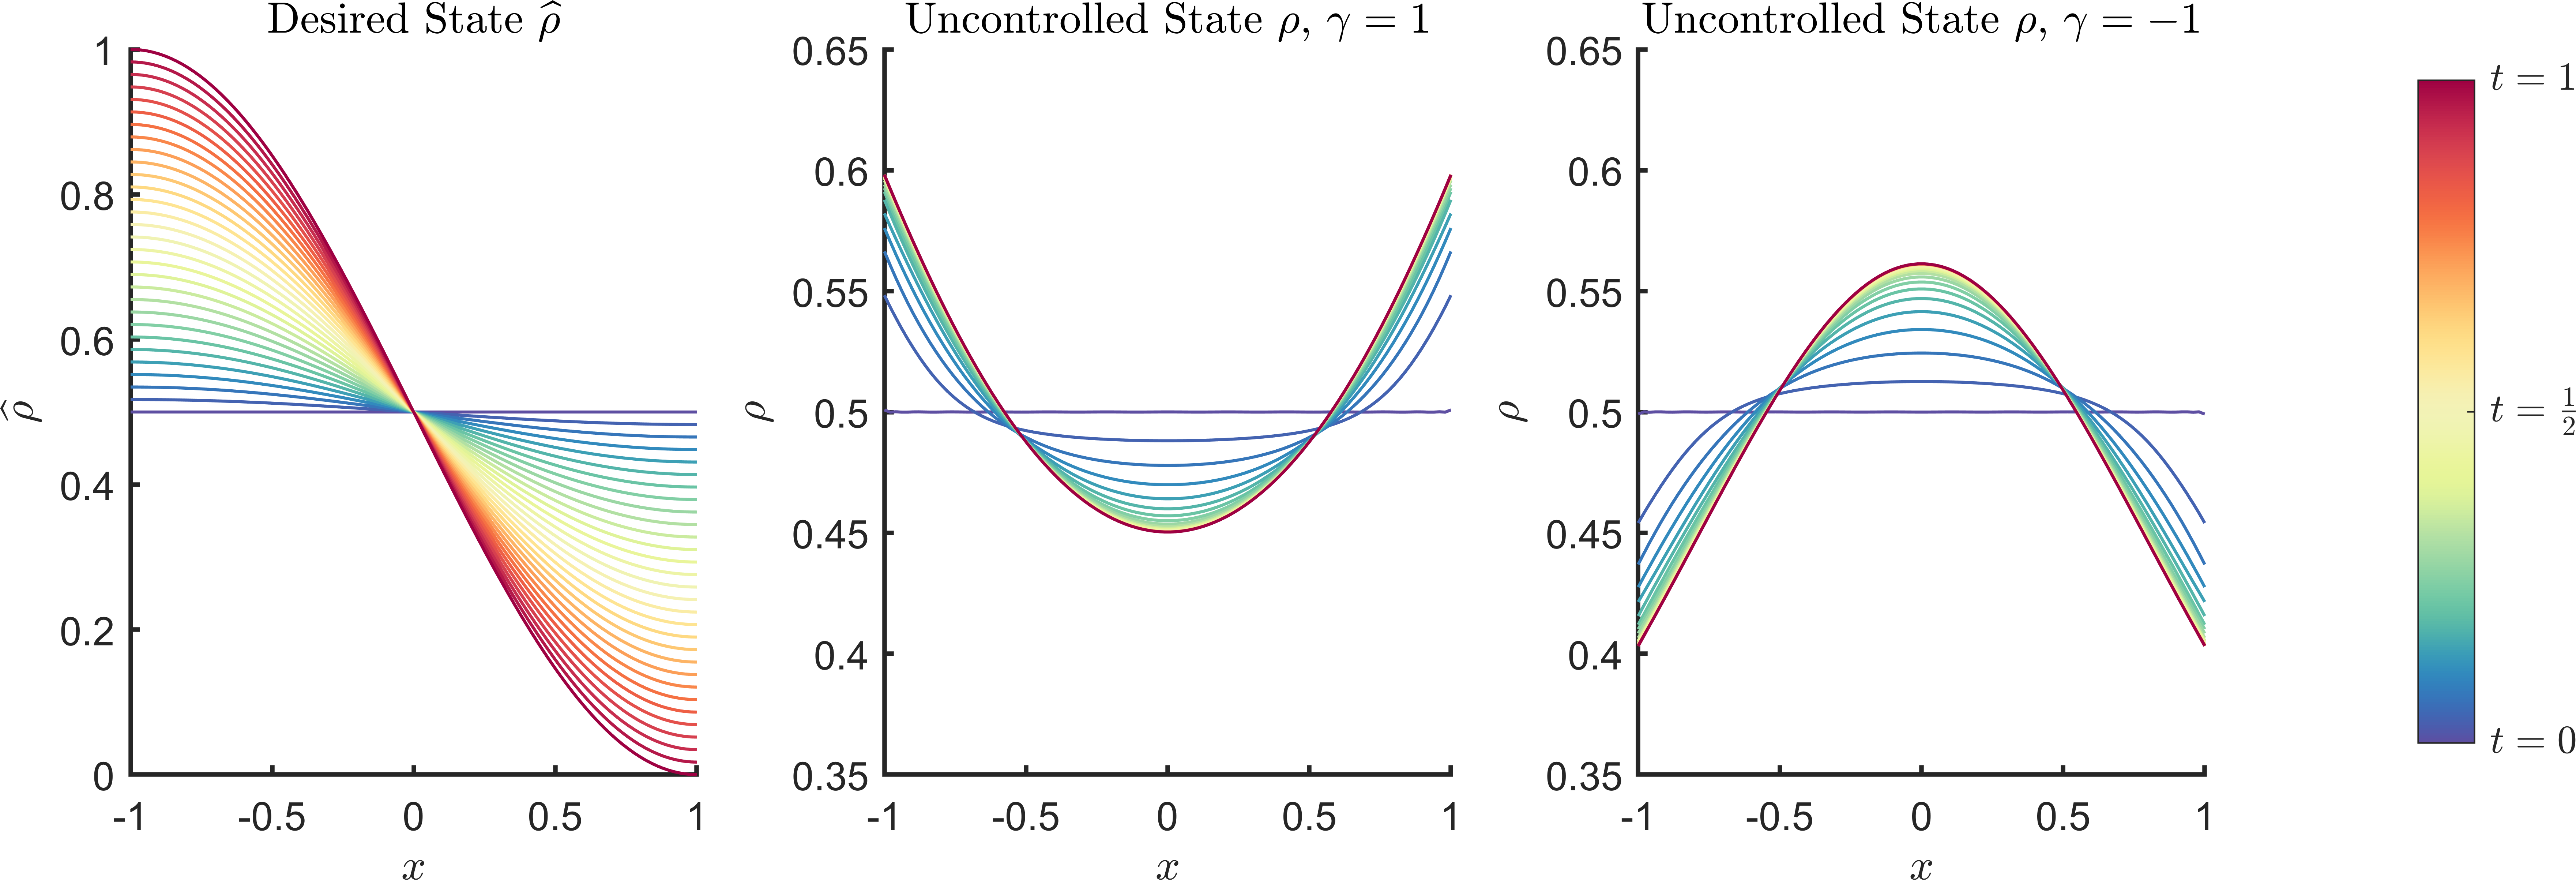
\includegraphics[scale=0.05]{Figure1.png}
	\caption{Example 1, desired state $\widehat \rho$ and uncontrolled state $\rho$ at $\gamma =1$ and $\gamma =-1$}
	\label{Ex12DN1}
\end{figure}
\begin{figure}[h]
	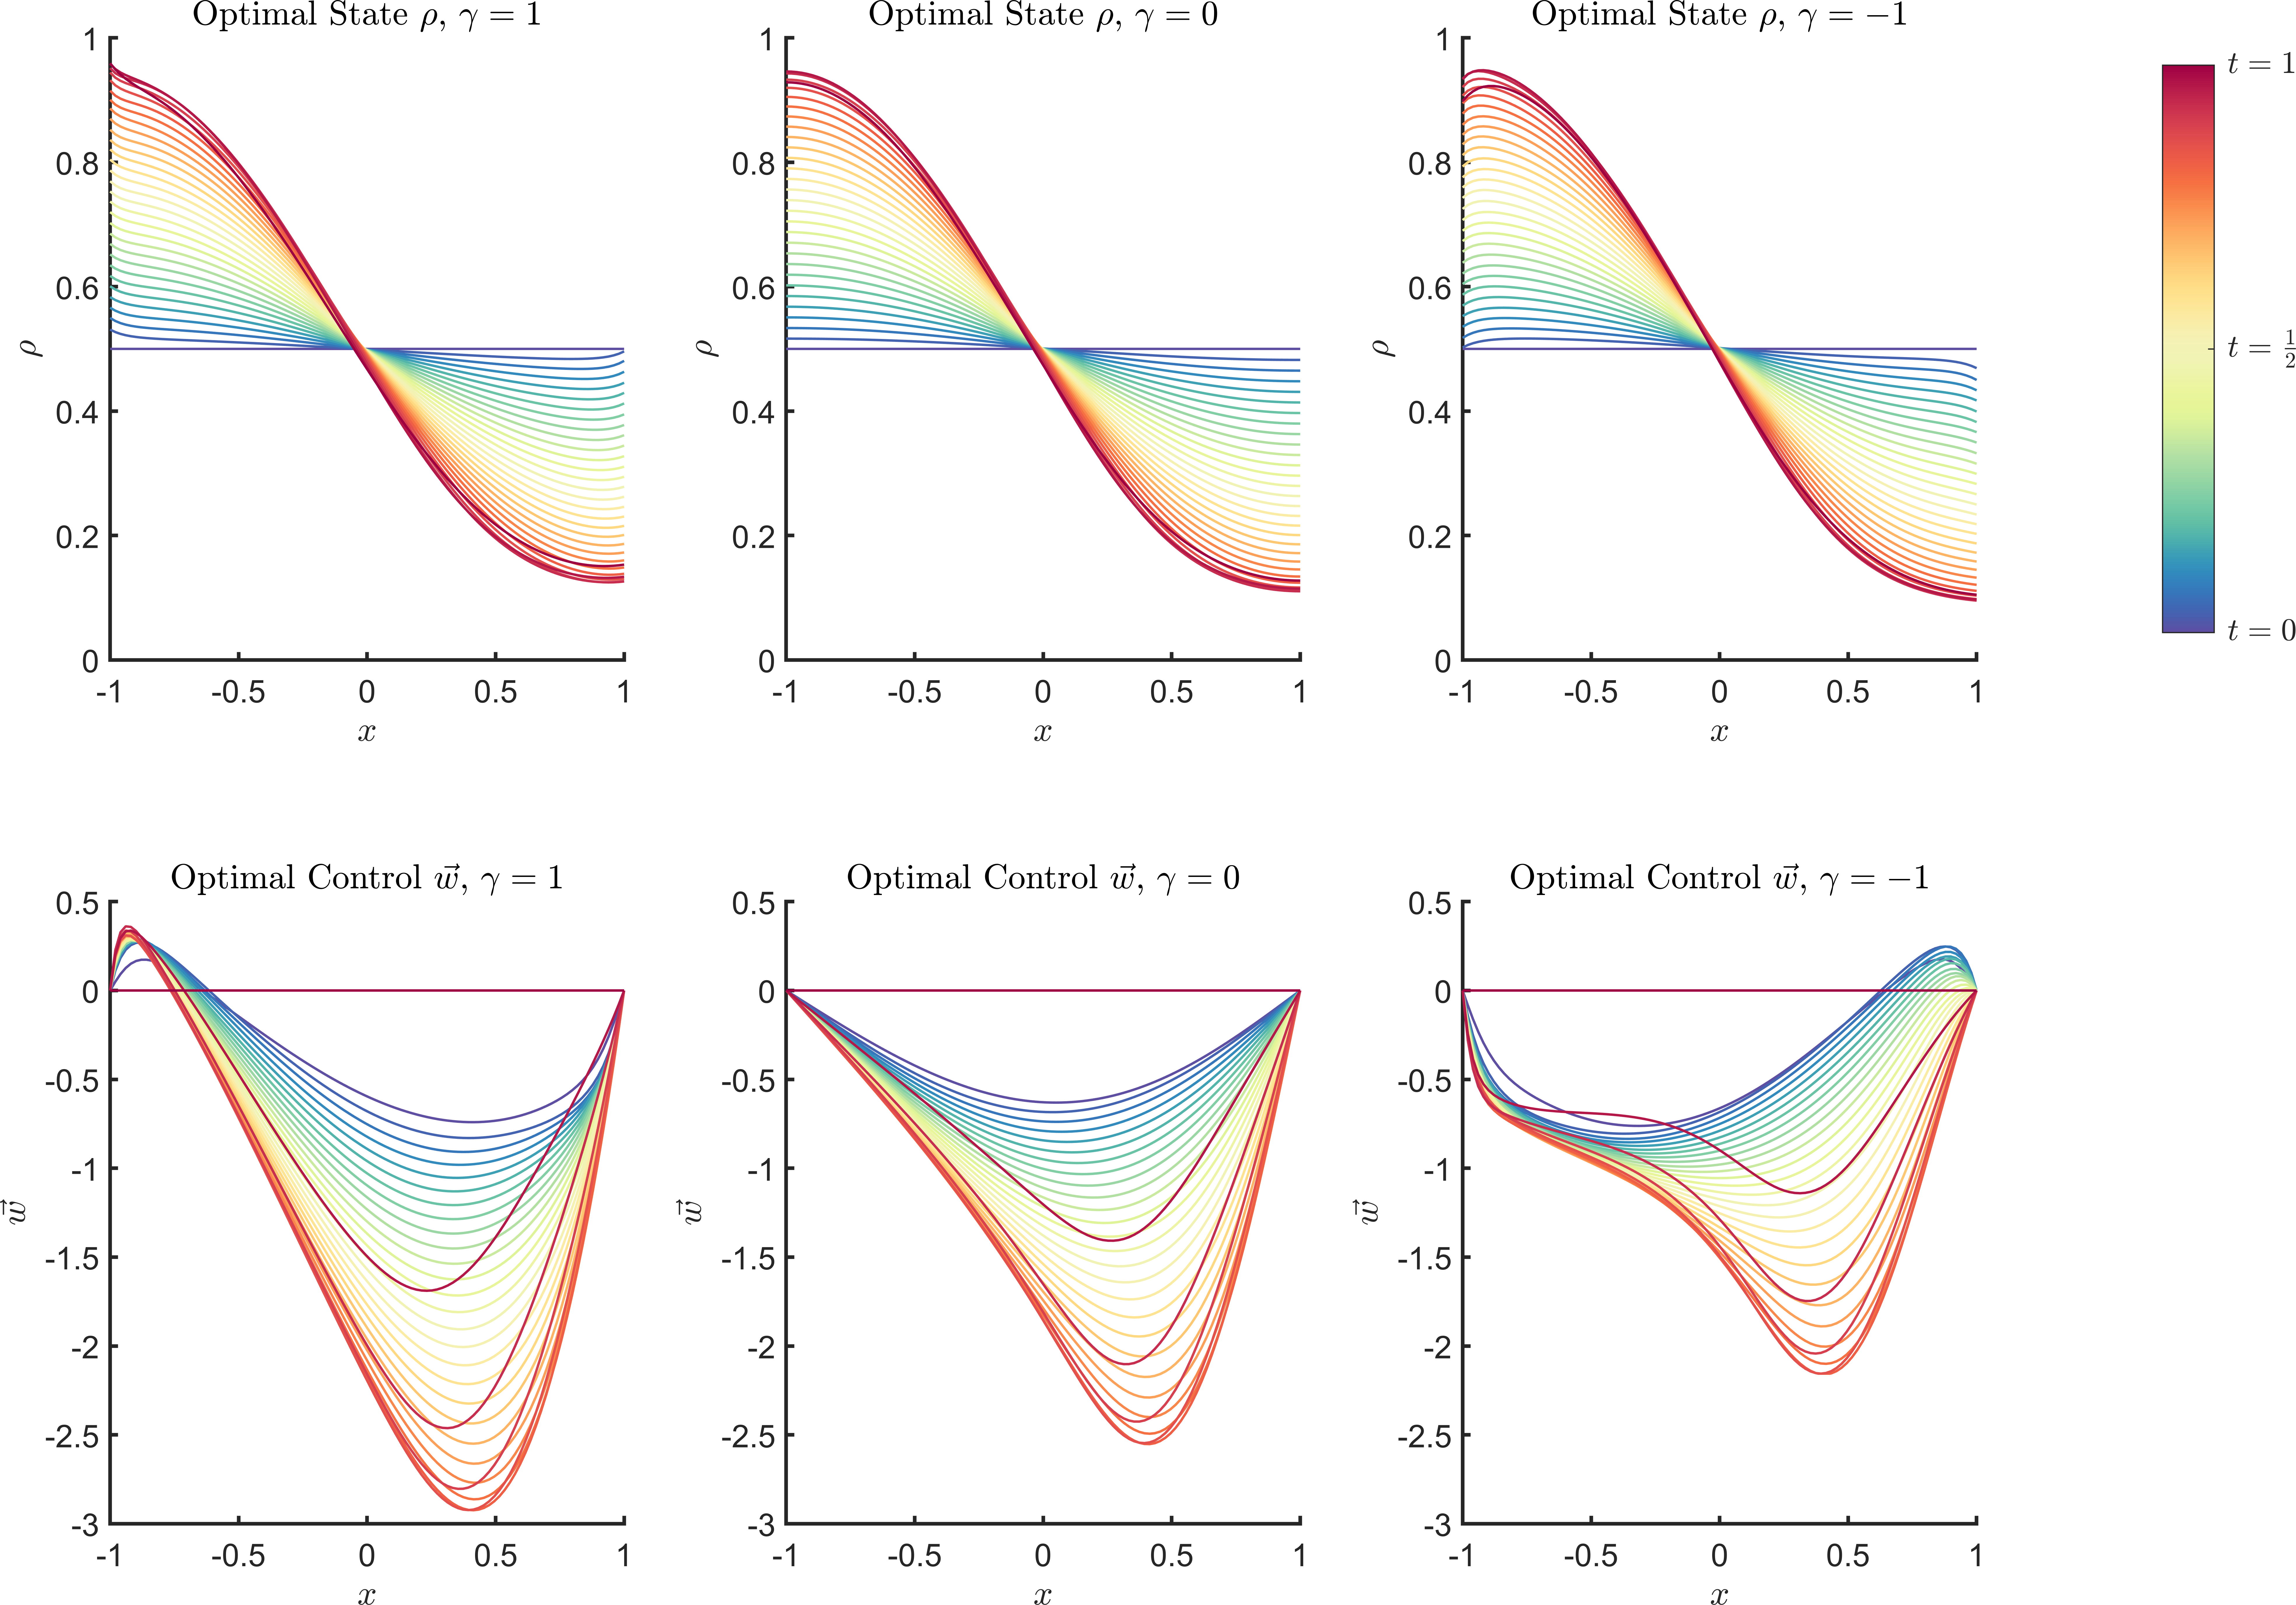
\includegraphics[scale=0.05]{Figure2.png}
	\caption{Example 1, optimal state $\rho$ and the corresponding optimal control $\vec{w}$ for $\gamma = 1,0,-1$, $\beta = 10^{-3}$.}
	\label{Ex12DN2}
\end{figure}

\begin{table}
\begin{tabular}{ | c | c || c | c | c | c ||}
\hline
\multicolumn{2}{|c||}{}& $\beta = 10^{-3}$ & $\beta = 10^{-1}$ & $\beta = 10^{1}$ & $\beta = 10^{3}$  \\
\hline
\hline
 & $\mathcal{J}_{uc}$ & $\numprint{0.0438}$ & $\numprint{0.0438}$ & $\numprint{0.0438}$ & $\numprint{0.0438}$ \\
$\kappa= \numprint{-1}$  & $\mathcal{J}_c$ & $\numprint{0.0011}$ & $\numprint{0.0267}$ & $\numprint{0.0435}$ & $\numprint{0.0438}$ \\
& \texttt{Iter} & $\numprint{670}$ & $\numprint{650}$ & $\numprint{449}$ & $\numprint{1}$ \\
\hline
 & $\mathcal{J}_{uc}$ & $\numprint{0.0417}$ & $\numprint{0.0417}$ & $\numprint{0.0417}$ & $\numprint{0.0417}$ \\
$\kappa= \numprint{0}$  & $\mathcal{J}_c$ & $\numprint{0.0014}$ & $\numprint{0.0283}$ & $\numprint{0.0415}$ & $\numprint{0.0417}$ \\
& \texttt{Iter} & $\numprint{665}$ & $\numprint{656}$ & $\numprint{434}$ & $\numprint{1}$ \\
\hline
 & $\mathcal{J}_{uc}$ & $\numprint{0.0434}$ & $\numprint{0.0434}$ & $\numprint{0.0434}$ & $\numprint{0.0434}$ \\
$\kappa= \numprint{1}$  & $\mathcal{J}_c$ & $\numprint{0.0020}$ & $\numprint{0.0322}$ & $\numprint{0.0432}$ & $\numprint{0.0434}$ \\
& \texttt{Iter} & $\numprint{654}$ & $\numprint{682}$ & $\numprint{422}$ & $\numprint{1}$ \\
\hline
\end{tabular}
\caption{Example 1: Uncontrolled cost $\mathcal{J}_{uc}$, optimal control cost $\mathcal{J}_{c}$, and number of iterations \emph{\texttt{Iter}}, for a range of $\kappa$ and $\beta$ values.}
\label{TabS5:Prob1}
\end{table} %\label{TabS5:Prob1}


\subsubsection{Neumann boundary conditions, Example 2} 
The chosen inputs for Example 2 are:
\begin{align*}
&\widehat \rho = \bigg(\frac{1}{2}\cos(\pi y) + \frac{1}{2}\bigg)(1-t) + t\bigg(-\frac{1}{2}\cos(2 \pi y) + \frac{1}{2}\bigg),\\
&\rho_{0} = \frac{1}{2}\cos(\pi y) + \frac{1}{2},\ \
\adj_{T} = 0,\ \
\vec{w} = \vec{0},\ \
f =0,\ \
V_{ext} =0.
\end{align*}
In Table \ref{TabS5:Prob2} the results for Example 2 are displayed. These are comparable with the results for Example 1, in the effect of $\beta$ and the number of iterations. In all three configurations of the interaction term, the control is focussed on transporting the mass from the middle of the domain onto two piles centred at $x=-0.5$ and $x=0.5$. In Figure \ref{Ex22DN1}, the desired state $\widehat \rho$, the optimal state $\rho$ and the optimal control $\vec{w}$ are displayed for $\beta = 10^{-3}$ and $\gamma = 1$, and compared to Example 3 below. Here, the number of points is chosen to be $N=40$ and $n=30$ (instead of $N=30$ and $n=20$), due to the steep gradients of the desired state.
\begin{figure}[h]
	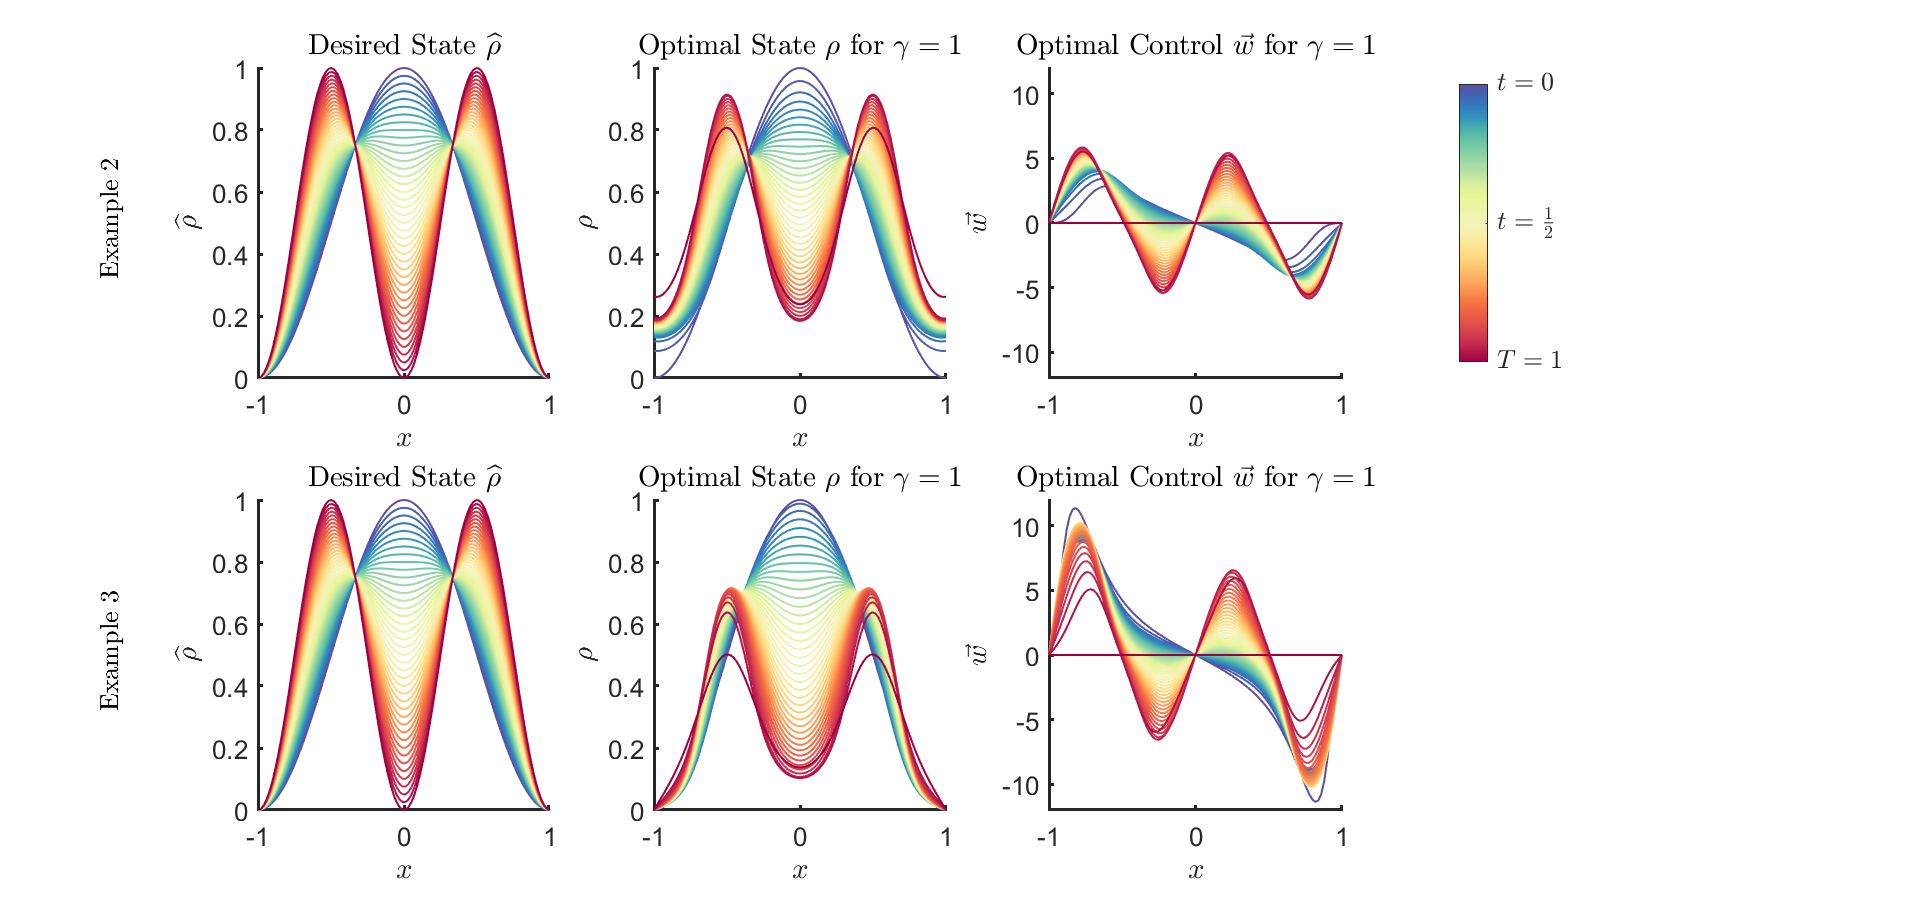
\includegraphics[scale=0.05]{Figure3.png}
	\caption{Example 2/ Example 3, desired state $\widehat \rho$, optimal state $\rho$ and corresponding optimal control $\vec{w}$, $\beta = 10^{-3}$, $\gamma = 1$.}
	\label{Ex22DN1}
\end{figure}

\begin{table}
\begin{tabular}{ | c | c || c | c | c | c ||}
\hline
\multicolumn{2}{|c||}{}& $\beta = 10^{-3}$ & $\beta = 10^{-1}$ & $\beta = 10^{1}$ & $\beta = 10^{3}$  \\
\hline
\hline
 & $\mathcal{J}_{uc}$ & $\numprint{0.0536}$ & $\numprint{0.0536}$ & $\numprint{0.0536}$ & $\numprint{0.0536}$ \\
$\kappa= \numprint{-1}$  & $\mathcal{J}_c$ & $\numprint{0.0096}$ & $\numprint{0.0492}$ & $\numprint{0.0535}$ & $\numprint{0.0536}$ \\
& \texttt{Iter} & $\numprint{715}$ & $\numprint{767}$ & $\numprint{367}$ & $\numprint{1}$ \\
\hline
 & $\mathcal{J}_{uc}$ & $\numprint{0.0669}$ & $\numprint{0.0669}$ & $\numprint{0.0669}$ & $\numprint{0.0669}$ \\
$\kappa= \numprint{0}$  & $\mathcal{J}_c$ & $\numprint{0.0109}$ & $\numprint{0.0603}$ & $\numprint{0.0668}$ & $\numprint{0.0669}$ \\
& \texttt{Iter} & $\numprint{714}$ & $\numprint{770}$ & $\numprint{390}$ & $\numprint{1}$ \\
\hline
 & $\mathcal{J}_{uc}$ & $\numprint{0.0839}$ & $\numprint{0.0839}$ & $\numprint{0.0839}$ & $\numprint{0.0839}$ \\
$\kappa= \numprint{1}$  & $\mathcal{J}_c$ & $\numprint{0.0125}$ & $\numprint{0.0748}$ & $\numprint{0.0838}$ & $\numprint{0.0839}$ \\
& \texttt{Iter} & $\numprint{713}$ & $\numprint{773}$ & $\numprint{403}$ & $\numprint{1}$ \\
\hline
\end{tabular}
\caption{Example 2: Cost when $\vec{w}=\vec{0}$, optimal control cost, and iterations required, for a range of $\kappa$, $\beta$.}
\label{TabS5:Prob2}
\end{table} %\label{TabS5:Prob2a}


\subsubsection{Dirichlet boundary conditions, Example 3} 
The inputs for this example are:
\begin{align*}
&\widehat \rho = \bigg(\frac{1}{2}\cos(\pi y) + \frac{1}{2}\bigg)(1-t) + t\bigg(-\frac{1}{2}\cos(2 \pi y) + \frac{1}{2}\bigg),\\
&\rho_{0} = \frac{1}{2}\cos(\pi y) + \frac{1}{2},\ \
\adj_{T} = 0,\ \
\vec{w} = \vec{0},\ \
f =0,\ \
V_{ext} =0.
\end{align*}
Table \ref{TabS5:Prob3} presents the results for this example, for a range of $\beta$ values and different interaction strengths. The observations are in line with those in Example 1 and 2. In particular, $ \widehat \rho$ and $\rho_0$ coincide with those of the problem with Neumann boundary conditions in Example 2. A comparison between the two examples is illustrated in Figure \ref{Ex22DN1}. Both the optimal state $\rho$ and the optimal control are qualitatively different when considering Dirichlet boundary conditions over Neumann conditions. The numerical result for this example was achieved with $N=40$ and $n = 30$, rather than with $N=30$ and $n=20$. This indicates that the Dirichlet boundary conditions are harder to apply in this problem, due to the steep shape of the desired state. This steepness is somewhat less impactful in Example 2, where the desired state is not closely matched by the optimal state at the boundaries. In Example 3, while the optimal state matches the desired state perfectly at the boundary, the peaks of the desired state are matched less closely. In Figure \ref{Ex22DN1}, this can be confirmed by considering the control plots. The optimal control for Example 3 is larger than for Example 2, specifically between the boundaries of the domain and the peaks of the desired state, indicating difficulties in this region.
\begin{table}
\begin{tabular}{ ||c|| c | c | c | c | c ||}
\hline
& & $\beta = 10^{-3}$ & $\beta = 10^{-1}$ & $\beta = 10^{1}$ & $\beta = 10^{3}$  \\
\hline
 & $J_{uc}$ & $\numprint{1.4165e-1}$ & $\numprint{1.4165e-1}$ & $\numprint{1.4165e-1}$ & $\numprint{1.4165e-1}$ \\
$\gamma= \numprint{-1}$  & $J_c$ & $\numprint{3.5594e-2}$ & $\numprint{1.3270e-1}$ & $\numprint{1.4155e-1}$ & $\numprint{1.4165e-1}$ \\
& $Iter.$ & $\numprint{944}$ & $\numprint{816}$ & $\numprint{437}$ & $\numprint{1}$ \\
\hline
 & $J_{uc}$ & $\numprint{1.5452e-1}$ & $\numprint{1.5452e-1}$ & $\numprint{1.5452e-1}$ & $\numprint{1.5452e-1}$ \\
$\gamma= \numprint{0}$  & $J_c$ & $\numprint{3.8023e-2}$ & $\numprint{1.4549e-1}$ & $\numprint{1.5442e-1}$ & $\numprint{1.5452e-1}$ \\
& $Iter.$ & $\numprint{940}$ & $\numprint{825}$ & $\numprint{440}$ & $\numprint{1}$ \\
\hline
 & $J_{uc}$ & $\numprint{1.6610e-1}$ & $\numprint{1.6610e-1}$ & $\numprint{1.6610e-1}$ & $\numprint{1.6610e-1}$ \\
$\gamma= \numprint{1}$  & $J_c$ & $\numprint{4.1143e-2}$ & $\numprint{1.5751e-1}$ & $\numprint{1.6601e-1}$ & $\numprint{1.6610e-1}$ \\
& $Iter.$ & $\numprint{932}$ & $\numprint{827}$ & $\numprint{440}$ & $\numprint{1}$ \\
\hline
\end{tabular}
\caption{Problem 3 ($n = 30,N = 40$)}
\label{TabS5:Prob3}
\end{table} %\label{TabS5:Prob3}


%\subsubsection{Neumann boundary conditions, Symmetric Example 1}
%Consider the following symmetric setup:
%\begin{align*}
%\widehat \rho &= \frac{1}{2}(1-t) + t\frac{1}{4}(\cos(\pi y)+2),\\
%\rho_{0} &= \frac{1}{2},\  \ q_{T} = 0, \ \ \vec{w} = \vec{0}, \ \  f =0, \ \ V_{ext} =0.
%\end{align*}
%Table \ref{TabNFlowAddEx1} summarizes the results for this example.The attractive interaction term causes $\rho$ to move towards the centre of the domain. Since $\widehat \rho$ is also centred in the domain, $J_{uc}$ is small for $\gamma =-1$ in comparison to the problems with $\gamma =0$ and $\gamma =1$. This example illustrates that the particle interaction term can have a significant impact on the optimization problem considered. 
%
%
%
%
%\subsubsection{Neumann boundary conditions, Symmetric Example 2}
%Consider the following symmetric setup, which is the opposite of the first symmetric example:
%\begin{align*}
%\widehat \rho &= \frac{1}{2}(1-t) + t\frac{1}{4}(-\cos(\pi y)+2),\\
%\rho_{0} &= \frac{1}{2},\ \
%q_{T} = 0,\ \
%\vec{w} = \vec{0},\ \
%f =0,\ \
%V_{ext} =0.
%\end{align*}
%This example can be compared to the Symmetric Example 1. Here, the desired state is having $\rho$ clustered at both boundaries, which is similar to the effect of the repulsive interaction term $\gamma = 1$. Therefore, for this choice of interaction term, the value of the cost functional $J_{uc}$ is smaller than the one for $\gamma = 0$ and $\gamma = -1$. This is the opposite to the observation made in the Symmetric Example 1, which is to be expected, given the two choices of desired state.


\subsection{Linear control problems with an additional nonlocal integral term}
In this section, examples of solving Problem \eqref{AdvDiff_Linear} with both 'no-flux type' boundary conditions \eqref{NoFlux_Linear} and Dirichlet boundary conditions \eqref{Dirichlet}.
\subsubsection{Dirichlet boundary conditions, Example 4}
The inputs for this example are:
\begin{align*}
&\widehat \rho = (1 - t)\bigg(\frac{1}{2}\cos(\pi y) + \frac{1}{2}\bigg)  + t\bigg(-\frac{1}{2}\cos(\pi y) + \frac{1}{2}\bigg),\\
&\rho_{0} = \frac{1}{2}\cos(\pi y) + \frac{1}{2},\ \
\adj_{T} = 0,\ \
{w} = 0,\ \
f =0, \ \
V_{ext} =\frac{1}{2}\left((x + 0.3)^2 - 0.2\right)\left((x-0.4)^2 - 0.3\right).
\end{align*}
In Table \ref{TabS5:Prob4} the results for Example 4 for a range of parameter values can be found. The results are qualitatively similar to the previous examples, but the control is applied linearly in this example. Note that here $\lambda = 0.005$, since $V_{{ext}}$ causes the numerical computations to be more challenging.
\begin{table}
\begin{tabular}{ | c | c || c | c | c | c ||}
\hline
\multicolumn{2}{|c||}{}& $\beta = 10^{-3}$ & $\beta = 10^{-1}$ & $\beta = 10^{1}$ & $\beta = 10^{3}$  \\
\hline
\hline
 & $\mathcal{J}_{uc}$ & $\numprint{0.1394}$ & $\numprint{0.1394}$ & $\numprint{0.1394}$ & $\numprint{0.1394}$ \\
$\kappa= \numprint{-1}$  & $\mathcal{J}_c$ & $\numprint{0.0183}$ & $\numprint{0.0862}$ & $\numprint{0.1384}$ & $\numprint{0.1394}$ \\
& \texttt{Iter} & $\numprint{1575}$ & $\numprint{1486}$ & $\numprint{1026}$ & $\numprint{117}$ \\
\hline
 & $\mathcal{J}_{uc}$ & $\numprint{0.1526}$ & $\numprint{0.1526}$ & $\numprint{0.1526}$ & $\numprint{0.1526}$ \\
$\kappa= \numprint{0}$  & $\mathcal{J}_c$ & $\numprint{0.0183}$ & $\numprint{0.0983}$ & $\numprint{0.1516}$ & $\numprint{0.1526}$ \\
& \texttt{Iter} & $\numprint{1582}$ & $\numprint{1474}$ & $\numprint{1023}$ & $\numprint{113}$ \\
\hline
 & $\mathcal{J}_{uc}$ & $\numprint{0.1645}$ & $\numprint{0.1645}$ & $\numprint{0.1645}$ & $\numprint{0.1645}$ \\
$\kappa= \numprint{1}$  & $\mathcal{J}_c$ & $\numprint{0.0189}$ & $\numprint{0.1103}$ & $\numprint{0.1635}$ & $\numprint{0.1645}$ \\
& \texttt{Iter} & $\numprint{1589}$ & $\numprint{1465}$ & $\numprint{1022}$ & $\numprint{112}$ \\
\hline
\end{tabular}
\caption{Example 4: Uncontrolled cost $\mathcal{J}_{uc}$, optimal cost $\mathcal{J}_{c}$, and number of iterations, for a range of $\kappa$ and $\beta$ values.}
\label{TabS5:Prob4}
\end{table} %\label{TabS5:Prob4}




\subsubsection{Neumann boundary conditions, Example 5}
The inputs for this example are:
\begin{align*}
&\widehat \rho = \frac{1}{2}(1-t) + t\frac{1}{2}(-\cos(\pi y) + 1),\\
&\rho_{0} = \frac{1}{2},\ \
\adj_{T} = 0,\ \
{w} = 0,\ \
f =0,\ \
V_{ext} =0.
\end{align*}
Table \ref{TabS5:Prob5} shows the results for Example 5. Note that for this example, when $\beta = 10^{-3}$, the mixing parameter $\lambda$ had to be set to $0.001$, to guarantee stable convergence of the method (why? explanation needed?).
Again, the only qualitative difference to interpreting the results is that the control is applied linearly.
\begin{table}
\begin{tabular}{ ||c|| c | c | c | c | c ||}
\hline
& & $\beta = 10^{-3}$ & $\beta = 10^{-1}$ & $\beta = 10^{1}$ & $\beta = 10^{3}$  \\
\hline
 & $J_{uc}$ & $\numprint{6.0640e-2}$ & $\numprint{6.0640e-2}$ & $\numprint{6.0640e-2}$ & $\numprint{6.0640e-2}$ \\
$\gamma= \numprint{-1}$  & $J_c$ & $\numprint{6.0180e-3}$ & $\numprint{5.5365e-2}$ & $\numprint{6.0592e-2}$ & $\numprint{6.0640e-2}$ \\
& $Iter.$ & $\numprint{7320}$ & $\numprint{7712}$ & $\numprint{3888}$ & $\numprint{1}$ \\
\hline
 & $J_{uc}$ & $\numprint{4.1667e-2}$ & $\numprint{4.1667e-2}$ & $\numprint{4.1667e-2}$ & $\numprint{4.1667e-2}$ \\
$\gamma= \numprint{0}$  & $J_c$ & $\numprint{4.5414e-3}$ & $\numprint{3.8334e-2}$ & $\numprint{4.1632e-2}$ & $\numprint{4.1667e-2}$ \\
& $Iter.$ & $\numprint{7271}$ & $\numprint{7614}$ & $\numprint{3643}$ & $\numprint{1}$ \\
\hline
 & $J_{uc}$ & $\numprint{2.8551e-2}$ & $\numprint{2.8551e-2}$ & $\numprint{2.8551e-2}$ & $\numprint{2.8551e-2}$ \\
$\gamma= \numprint{1}$  & $J_c$ & $\numprint{3.5942e-3}$ & $\numprint{2.6480e-2}$ & $\numprint{2.8529e-2}$ & $\numprint{2.8551e-2}$ \\
& $Iter.$ & $\numprint{7249}$ & $\numprint{7482}$ & $\numprint{3410}$ & $\numprint{1}$ \\
\hline
\end{tabular}
\caption{Problem 5}
\label{TabS5:Prob5}
\end{table} %\label{TabS5:Prob5}


\subsection{Nonlinear control problems with an additional nonlocal integral term in 2D}
In this section, two-dimensional examples are considered, to illustrate the fact that the application of the method differs very little from the one dimensional setting. The main difference is that in nonlinear control problems the control is a two-dimensional vector field. Furthermore, the number of spatial points increases from $N$ to $N_1\times N_2$, which makes computations much more costly. Compensating for this increased cost is one of the motivations to develop fast optimization solvers, such as the fixed point method introduced in Section \ref{sec:Method_Solver}.
\subsubsection{Neumann boundary conditions, Example 1}	
We have the following set up:
\begin{align*}
&\widehat \rho = \frac{1}{4}(1-t) + t\bigg(\frac{1}{4}\sin \bigg(\frac{\pi}{2}(x_1 - 2)\bigg)\sin \bigg(\frac{\pi}{2}(x_2 - 2)\bigg) + \frac{1}{4}\bigg),\\
&\rho_0 = \frac{1}{4},\ \
q_{T} = 0,\ \
\vec{w} = \vec{0},\ \
f =0,\ \
V_{ext} =0.
\end{align*}
This example is the two dimensional version of Example 1 in Section \ref{sec:Examples1d}. The results for this example are displayed in Table \ref{TabS5:Prob12D}. In Figures \ref{rhoHat2dEx2} it can be observed that as in Example 1 in Section \ref{sec:Examples1d}, the uncontrolled state forms a cluster in the centre of the domain, due to the attractive interactions. Figure \ref{rhoOpt2dEx2} shows the optimal state and control for different time points, for $\beta = 10^{-3}$ and $\gamma = -1$. Here, the control through a vector field illustrates why nonlinear control is called 'flow control'. 

\begin{table}
\begin{tabular}{ ||c|| c | c | c | c | c ||}
\hline
& & $\beta = 10^{-3}$ & $\beta = 10^{-1}$ & $\beta = 10^{1}$ & $\beta = 10^{3}$  \\
\hline
 & $\mathcal J_{\vec w = \vec 0}$ & $0.0113$ & $0.0113$ & $0.0113$ & $0.0113$ \\
$\kappa= -1$  & $\mathcal J_{Opt}$ & $0.0013$ & $0.0104$ & $0.0113$ & $0.0113$ \\
& $\text{Iterations}$ & $676$ & $700$ & $290$ & $1$ \\
\hline
\end{tabular}
\caption{Results for the test problem, with different $\beta$}
\label{TabS5:Prob12D}
\end{table} % \label{TabS5:Prob12D}

\begin{figure}[h]
	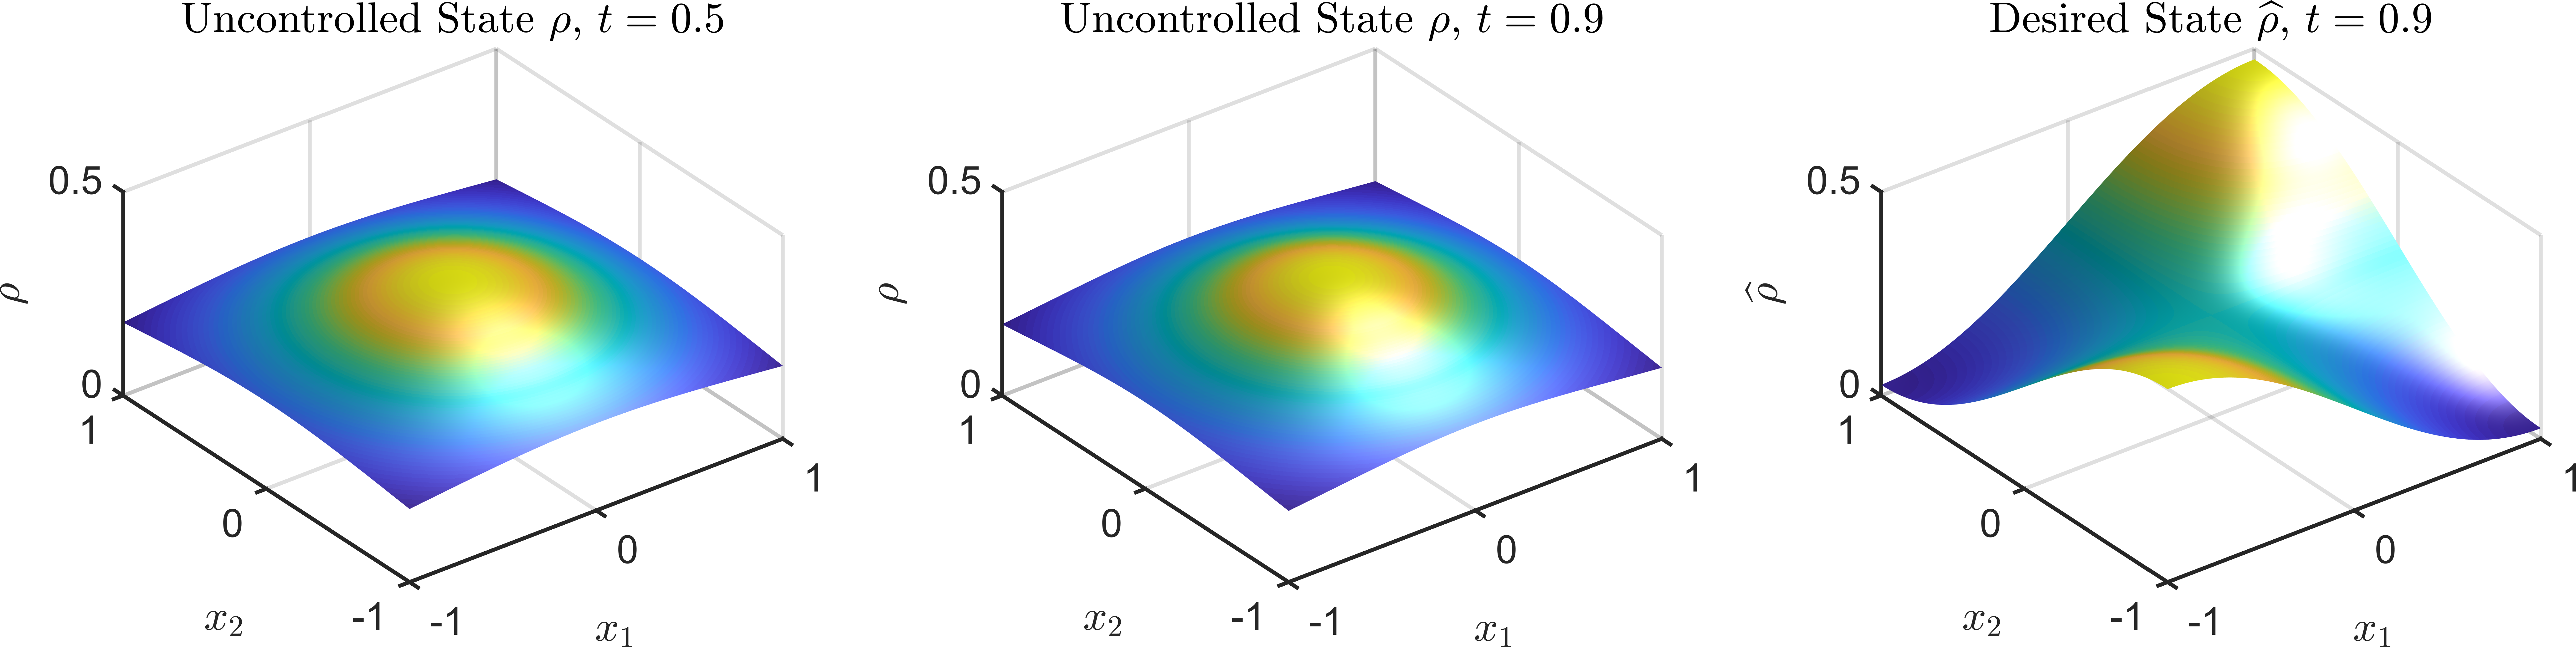
\includegraphics[scale=0.05]{Figure12D.png}
	\caption{2D Example 1, uncontrolled $\rho$ and $\widehat \rho$, $\beta = 10^{-3}$, $\gamma = -1$.}
	\label{rhoHat2dEx2}
\end{figure}
\begin{figure}[h]
	\includegraphics[scale=0.06]{Figure22D.png}
	\caption{2D Example 1, controlled $\rho$ and optimal control $\vec{w}$, $\beta = 10^{-3}$, $\gamma = -1$.}
	\label{rhoOpt2dEx2}
\end{figure}


\subsubsection{Neumann boundary conditions, Example 2}	
Here, we have:
\begin{align*}
&\widehat \rho = \frac{1}{4}(1-t) + t\frac{1}{0.9921}e^{-3((y_1+0.2)^2 + (y_2+0.2)^2))},\\
&\rho_0 = \frac{1}{4},\ \
q_{T} = 0,\ \
\vec{w} = \vec{0},\ \
f =0,\\
&V_{ext} =\left((x_1 + 0.3)^2 - 1\right)\left((x_1-0.4)^2 - 0.5\right)
\left((x_2 + 0.3)^2 - 1\right)\left((x_2-0.4)^2 - 0.5\right).
\end{align*}
The numerical results for this example are displayed in Table \ref{TabS5:Prob22D}. In figures \ref{rhoHat2dEx4} and \ref{rhoOpt2dEx4} the results are illustrated for $\beta = 10^{-3}$ and $\gamma = -1$. It can be observed very clearly that the control is driving the particle distribution to the desired state. It is noticeable that the control does not act uniformly around the peak of the desired state, but also acts strongly in the area between the location of the desired peak and the point $(-1,1)$. This is due to the external potential being steep in this area and more control is needed to reach the desired state than in other parts of the domain.

\begin{table}
\begin{tabular}{ | c | c || c | c | c | c ||}
\hline
\multicolumn{2}{|c||}{}& $\beta = 10^{-3}$ & $\beta = 10^{-1}$ & $\beta = 10^{1}$ & $\beta = 10^{3}$  \\
\hline
\hline
 & $\mathcal{J}_{uc}$ & $\numprint{0.0378}$ & $\numprint{0.0378}$ & $\numprint{0.0378}$ & $\numprint{0.0378}$ \\
$\kappa= \numprint{-1}$  & $\mathcal{J}_c$ & $\numprint{0.0017}$ & $\numprint{0.0312}$ & $\numprint{0.0377}$ & $\numprint{0.0378}$ \\
& \texttt{Iter} & $\numprint{691}$ & $\numprint{736}$ & $\numprint{347}$ & $\numprint{1}$ \\
\hline
 & $\mathcal{J}_{uc}$ & $\numprint{0.0478}$ & $\numprint{0.0478}$ & $\numprint{0.0478}$ & $\numprint{0.0478}$ \\
$\kappa= \numprint{0}$  & $\mathcal{J}_c$ & $\numprint{0.0064}$ & $\numprint{0.0450}$ & $\numprint{0.0478}$ & $\numprint{0.0478}$ \\
& \texttt{Iter} & $\numprint{718}$ & $\numprint{784}$ & $\numprint{343}$ & $\numprint{1}$ \\
\hline
 & $\mathcal{J}_{uc}$ & $\numprint{0.0526}$ & $\numprint{0.0526}$ & $\numprint{0.0526}$ & $\numprint{0.0526}$ \\
$\kappa= \numprint{1}$  & $\mathcal{J}_c$ & $\numprint{0.0137}$ & $\numprint{0.0514}$ & $\numprint{0.0526}$ & $\numprint{0.0526}$ \\
& \texttt{Iter} & $\numprint{735}$ & $\numprint{790}$ & $\numprint{338}$ & $\numprint{1}$ \\
\hline
\end{tabular}
\caption{2D Ex. 2: Uncontrolled cost $\mathcal{J}_{uc}$, optimal cost $\mathcal{J}_{c}$, and number of iterations, for a range of $\kappa$ and $\beta$ values.}
\label{TabS5:Prob22D}
\end{table} %\label{TabS5:Prob22D}

\begin{figure}[h]
	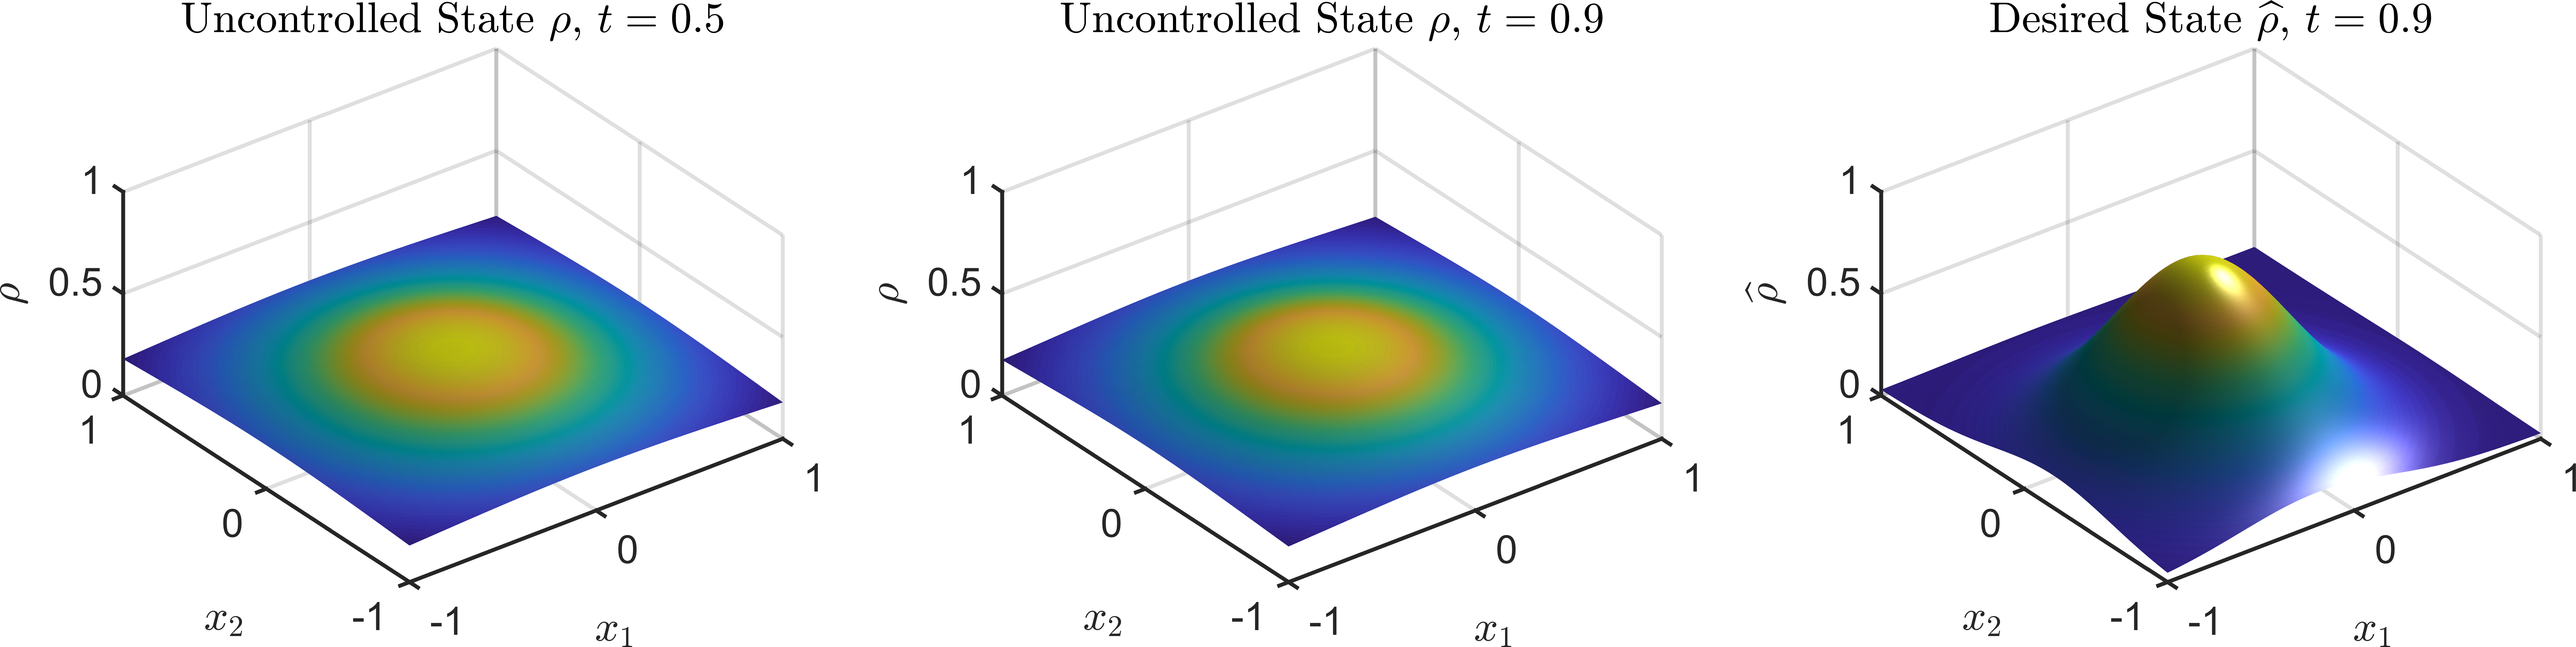
\includegraphics[scale=0.05]{Figure32D.png}
	\caption{2D Example 2: Uncontrolled $\rho$ and desired state $\widehat \rho$,  with $\beta = 10^{-3}$ and $\kappa = -1$. }
	\label{rhoHat2dEx4}
\end{figure}
\begin{figure}[h]
	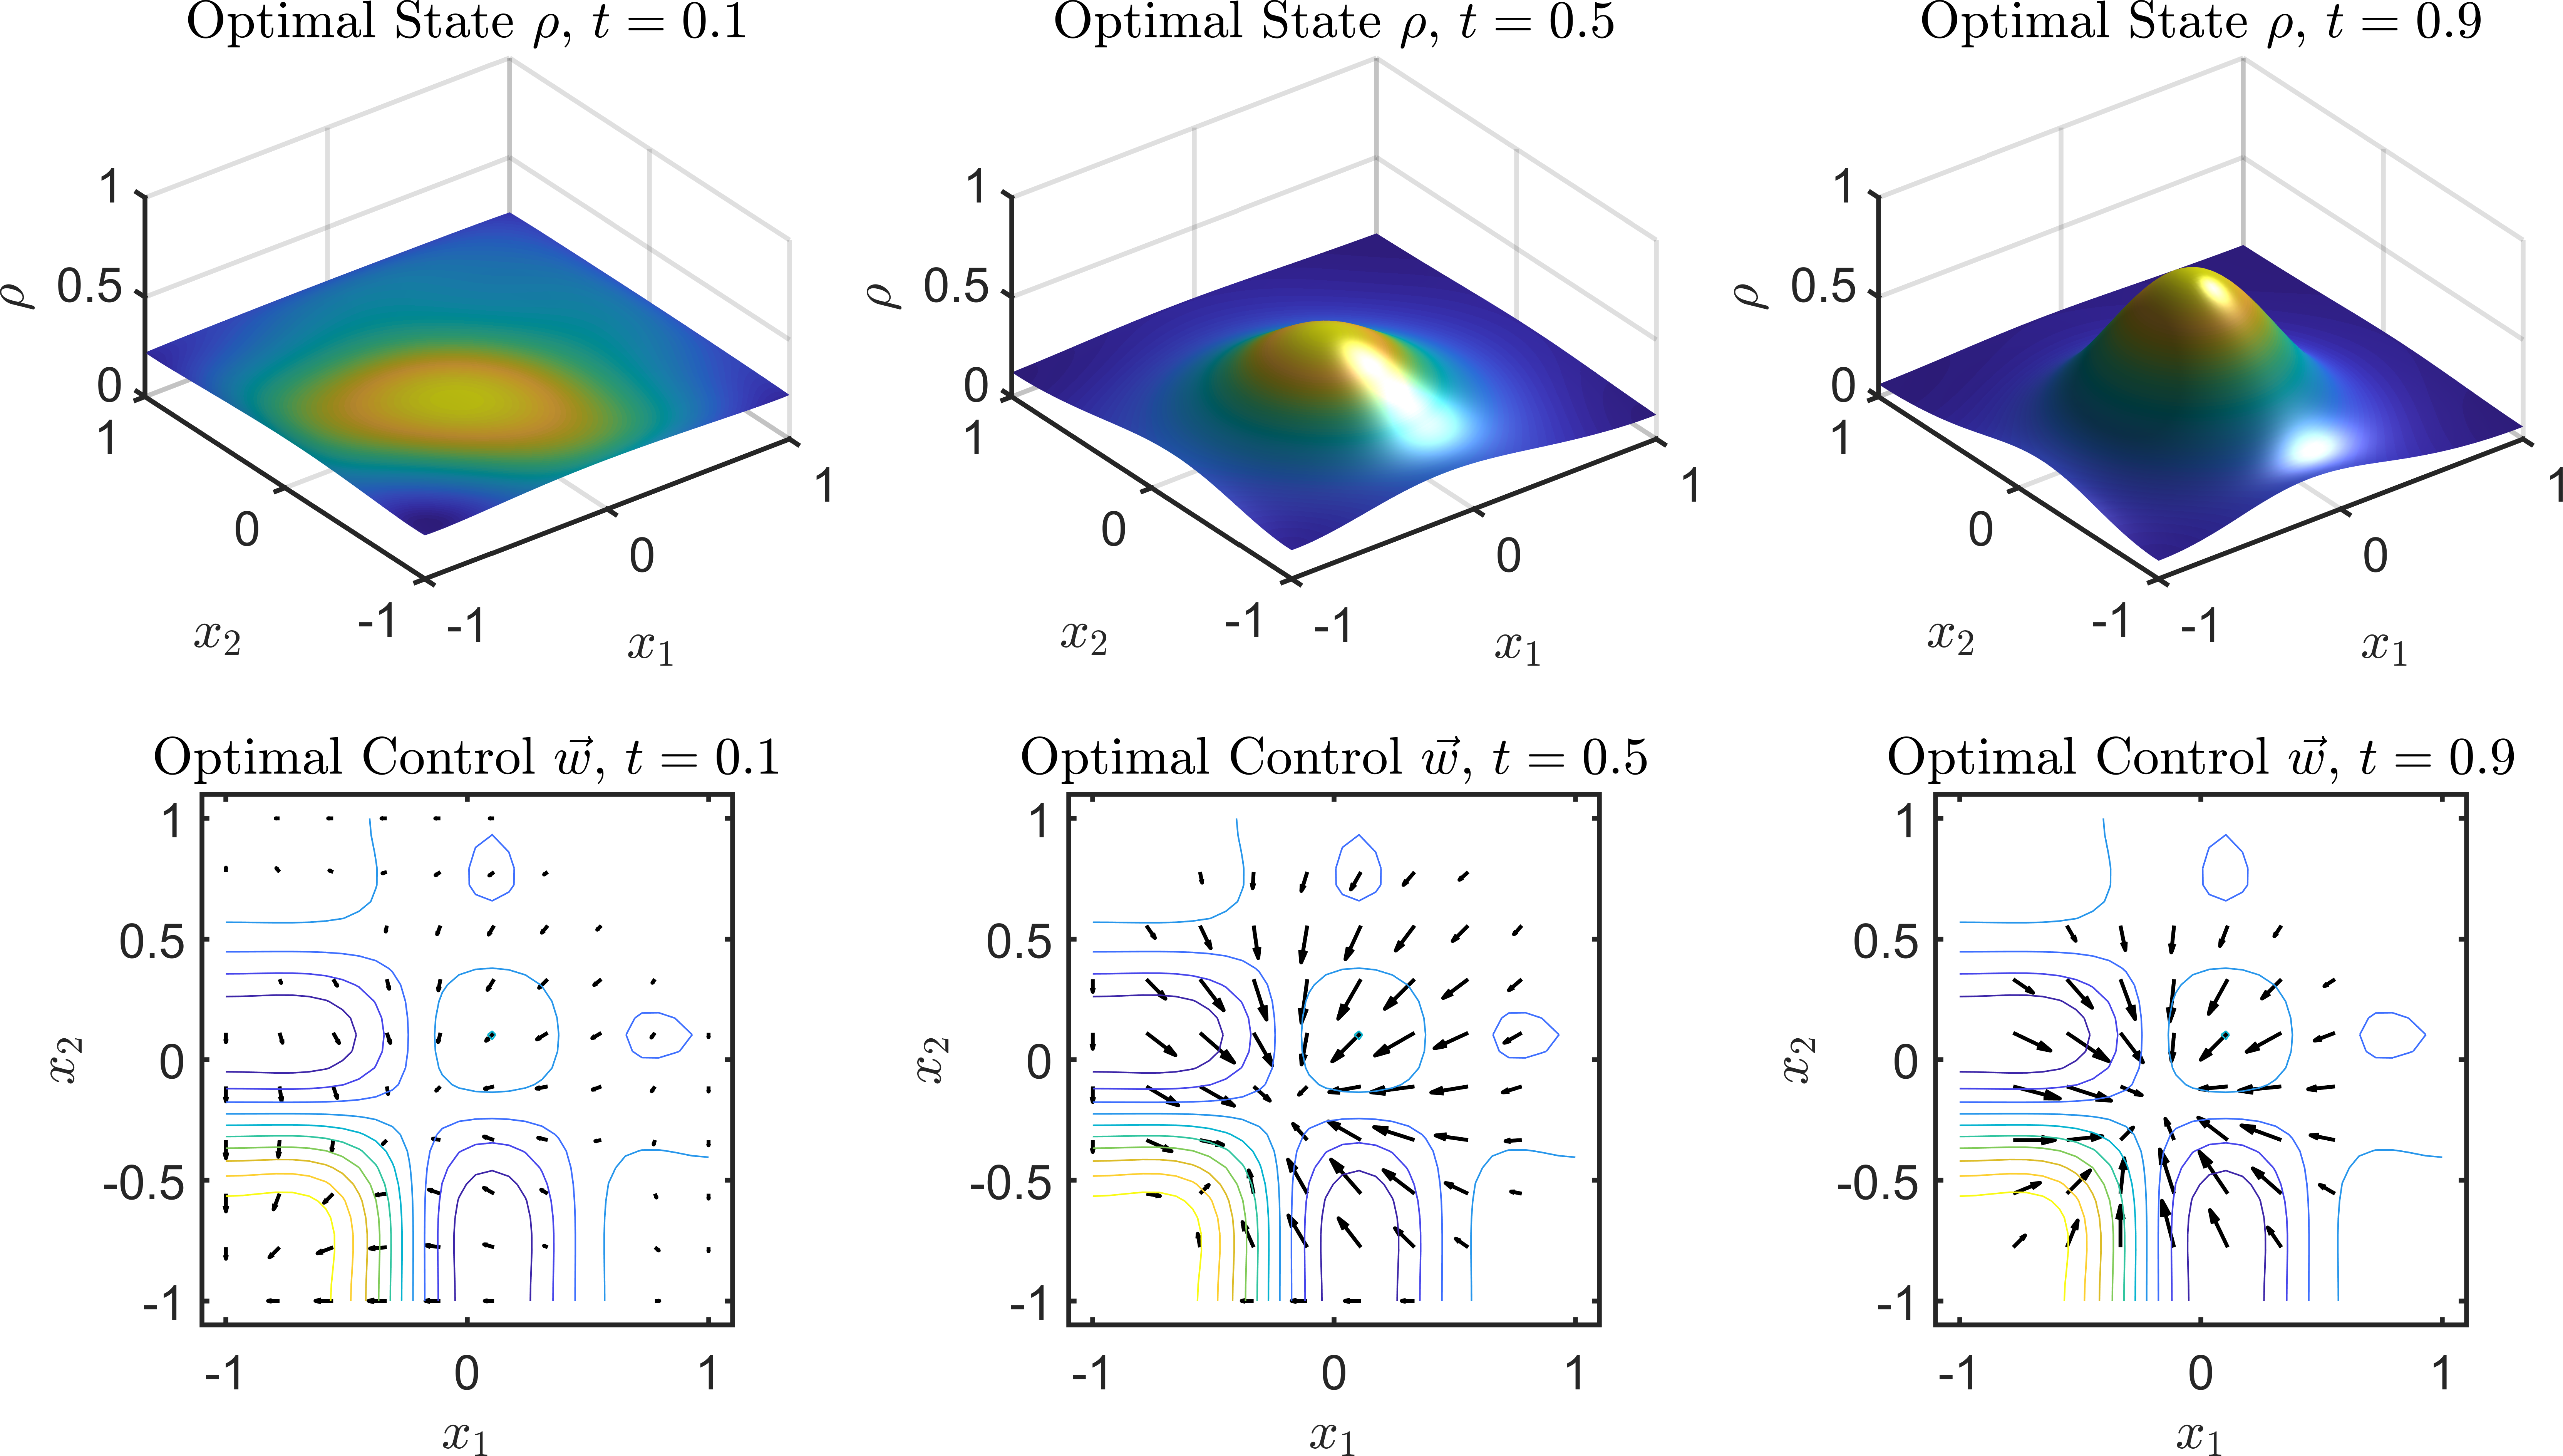
\includegraphics[scale=0.06]{Figure42D.png}
	\caption{2D Example 2: Optimal state $\rho$ and optimal control $\vec{w}$, with $\beta = 10^{-3}$ and $\kappa = -1$. A contour plot of the external potential $V^{\text{ext}}$ is superimposed on the control plots for reference.} 
	\label{rhoOpt2dEx4}
\end{figure}








\section{Concluding remarks}\label{sec:Conc}

Many extensions: ``final-time case'', different cost functionals, applications to opinion dynamics, flocking, swarming, robotics, ...


\vspace{0.75em}
\textbf{Acknowledgements.}~~
MA and JR are supported by The Maxwell Institute Graduate School in Analysis and
its Applications, a Centre for Doctoral Training funded by the UK Engineering and Physical Sciences
Research Council (EPSRC grant EP/L016508/01), the Scottish Funding Council, Heriot-Watt University, and
The University of Edinburgh.
%
BDG gratefully acknowledges support from the EPSRC grant EP/L025159/1.
%
JWP gratefully acknowledges support from the EPSRC Fellowship EP/M018857/2, the EPSRC grant EP/S027785/1, and a Fellowship from The Alan Turing Institute. 


\appendix

\section{Test problems with analytic solutions}\label{app:TestProblems}
+++ Need to double check the solutions, just in case! +++
In this appendix we present two test problems, posed on a two-dimensional domain $\Omega=(-1,1)^d$, where $d$ is the dimension of the problem.
Computing the errors between the given exact solution and the result of solving the uncontrolled PDE and the solution to the PDE-constrained optimization problem demonstrates the correct implementation of the algorithms at hand.  The error ($Err_{uc}$) between the exact solution for the state variable, $\rho_{Ex}$, and the uncontrolled state, $\rho_{uc}$, as well as the error ($Err_c$) between $\rho_{Ex}$ and the controlled state, $\rho_c$, are measured in a relative $L^2$ norm in space and in the $L_\infty$ norm in time, as introduced in Section \ref{sec:Method_Solver}.
\vspace{0.75em}

\textbf{\emph{-- \underline{Test Problem 1:}}}~~The following triplet $(\rho,\vec{w},\adj)$ form a solution to the first-order continuous optimality conditions derived for the advection--diffusion control problem \eqref{AdvDiff} with the zero Dirichlet boundary condition \eqref{Dirichlet}, with $d=2$ and $\gamma =0$:
\begin{align*}
\ \rho={}&2 \beta^{1/2}e^{t}\text{cos}\left(\frac{\pi{}x_1}{2}\right)\text{cos}\left(\frac{\pi{}x_2}{2}\right), \\
\ \vec{w}={}&\frac{\pi}{2} e^{t}(e^{T}-e^{t})\left[\text{sin}(\pi{}x_1)\text{cos}^2\left(\frac{\pi{}x_2}{2}\right),~\text{cos}^2\left(\frac{\pi{}x_1}{2}\right)\text{sin}(\pi{}x_2)\right]^T, \\
\ \adj={}&\beta^{1/2}(e^{T}-e^{t})\text{cos}\left(\frac{\pi{}x_1}{2}\right)\text{cos}\left(\frac{\pi{}x_2}{2}\right),
\end{align*}
where $\boldsymbol{x}=[x_1,x_2]^T$, and
\begin{align*}
\ \widehat{\rho}={}&\beta^{1/2} e^{t}\text{cos}\left(\frac{\pi{}x_1}{2}\right)\text{cos}\left(\frac{\pi{}x_1}{2}\right) -\beta^{1/2}\frac{\pi^2}{2}(e^{T}-e^{t})\text{cos}\left(\frac{\pi{}x_1}{2}\right)\text{cos}\left(\frac{\pi{}x_1}{2}\right) \\
\ &-\beta^{1/2}\frac{\pi^2}{2}e^{t}(e^{T}-e^{t})^2\left(\text{cos}\left(\frac{\pi{}x_1}{2}\right)\text{cos}\left(\frac{\pi{}x_2}{2}\right)\right)\left[\text{sin}^2\left(\frac{\pi{}x_1}{2}\right)\text{cos}^2\left(\frac{\pi{}x_2}{2}\right)+\text{cos}^2\left(\frac{\pi{}x_1}{2}\right)\text{sin}^2\left(\frac{\pi{}x_2}{2}\right)\right], \\
\ V_{\text{ext}}={}&0, \\
\ f={}&\beta^{1/2}\left(2+\pi^2\right)e^{t}\text{cos}\left(\frac{\pi{}x_1}{2}\right)\text{cos}\left(\frac{\pi{}x_1}{2}\right) \\
\ &+ 2\beta^{1/2}\pi^2 e^{2t}(e^{T}-e^{t})\\
&\left[\text{cos}^3\left(\frac{\pi{}x_1}{2}\right)\text{cos}^3\left(\frac{\pi{}x_2}{2}\right)
-\text{cos}^3\left(\frac{\pi{}x_1}{2}\right)\text{sin}^2\left(\frac{\pi{}x_2}{2}\right)\text{cos}\left(\frac{\pi{}x_2}{2}\right)-\text{cos}^3\left(\frac{\pi{}x_2}{2}\right)\text{sin}^2\left(\frac{\pi{}x_1}{2}\right)\text{cos}\left(\frac{\pi{}x_1}{2}\right)\right], \\
\ \rho_{0}={}&2 \beta^{1/2}\text{cos}\left(\frac{\pi{}x_1}{2}\right)\text{cos}\left(\frac{\pi{}x_2}{2}\right),
\end{align*}

+++ fix equations over size...+++
Table \ref{TabApp1} displays the results for Test Problem 1. It can be observed that the error for the uncontrolled problem ($Err_{uc}$), and the error for the optimal control problem ($Err_c$), coincide. This is because the same forward problem is solved in the first step of the fixed point algorithm as in solving the forward problem, when provided with the exact solution. 
++ Maybe change these tables to show the errors for $\adj$ and $w$ as well. ++

\begin{table}
\begin{tabular}{ ||c|| c | c | c | c | c ||}
\hline
& & $\beta = 10^{-3}$ & $\beta = 10^{-1}$ & $\beta = 10^{1}$ & $\beta = 10^{3}$  \\
\hline
 & $\mathcal{E}_\rho$ & $\numprint{3.8317e-8}$ & $\numprint{1.9069e-8}$ & $\numprint{1.3796e-8}$ & $\numprint{1.3553e-8}$ \\
 $N = $$\numprint{20}$, $n = $$\numprint{10}$  & $\mathcal{E}_\adj$ & $\numprint{2.5380e-8}$ & $\numprint{2.3672e-8}$ & $\numprint{4.6464e-8}$ & $\numprint{4.3990e-8}$ \\
& $\mathcal{E}_{\vec{w}}$ & $\numprint{4.1191e-6}$ & $\numprint{1.3377e-7}$ & $\numprint{4.1771e-8}$ & $\numprint{3.9213e-8}$ \\
\hline
 & $\mathcal{E}_\rho$ & $\numprint{3.9206e-8}$ & $\numprint{1.9023e-8}$ & $\numprint{1.4019e-8}$ & $\numprint{1.3863e-8}$ \\
 $N = $$\numprint{30}$, $n = $$\numprint{20}$  & $\mathcal{E}_\adj$ & $\numprint{3.9337e-8}$ & $\numprint{1.9436e-8}$ & $\numprint{1.3355e-8}$ & $\numprint{2.3327e-8}$ \\
& $\mathcal{E}_{\vec{w}}$ & $\numprint{6.4641e-6}$ & $\numprint{1.7823e-7}$ & $\numprint{2.0256e-8}$ & $\numprint{1.9866e-8}$ \\
\hline
 & $\mathcal{E}_\rho$ & $\numprint{3.8069e-8}$ & $\numprint{1.9085e-8}$ & $\numprint{1.4844e-8}$ & $\numprint{1.4700e-8}$ \\
 $N = $$\numprint{40}$, $n = $$\numprint{30}$  & $\mathcal{E}_\adj$ & $\numprint{3.6398e-8}$ & $\numprint{1.9813e-8}$ & $\numprint{1.5275e-8}$ & $\numprint{2.8452e-8}$ \\
& $\mathcal{E}_{\vec{w}}$ & $\numprint{5.9510e-6}$ & $\numprint{2.1531e-7}$ & $\numprint{2.3138e-8}$ & $\numprint{2.5820e-8}$ \\
\hline
\end{tabular}
\caption{Problem 1}
\label{TabA1:Prob1}
\end{table}
%
%\begin{table}
%	\begin{tabular}{ ||c|| c | c |c | c ||}
%		\hline
%		$\beta$ / $N_1 \times N_2$, $n$ & $10^{-3}$  & $10^{-1}$  & $10$ & $10^3$ \\ 
%		\hline 
%		&$Err_{uc} = 2.1694\times 10^{-7}$ &$Err_{uc} = 1.0138\times 10^{-8}$ &$Err_{uc} = 5.532\times 10^{-9}$ &$Err_{uc} = 5.514\times 10^{-9}$\\
%		20    &$Err_{c} = 0$ &$Err_{c} = 0$ &$Err_{c} = 0$ &$Err_{c} = 0$\\
%		\hline 
%		&$Err_{uc} =1.9745 \times 10^{-7}$ &$Err_{uc} =9.920\times 10^{-9}$ &$Err_{uc} = 5.759\times 10^{-9}$ &$Err_{uc} = 5.683 \times 10^{-9}$\\
%		30     &$Err_{c} =0$ &$Err_{c} = 0$ &$Err_{c} = 0$ &$Err_{c} = 0$\\
%		\hline 
%		&$Err_{uc} = 2.1367\times 10^{-7}$ &$Err_{uc} = 1.0051\times 10^{-8}$ &$Err_{uc} = 5.643\times 10^{-9}$ &$Err_{uc} = 5.611\times 10^{-9}$\\
%		40     &$Err_{c} = 0$ &$Err_{c} = 0$ &$Err_{c} = 0$ &$Err_{c} = 0$\\
%		\hline 
%	\end{tabular}
%	\caption{Update this table.}
%	\label{TabApp1}
%\end{table}




\vspace{0.75em}

\textbf{\emph{-- \underline{Test Problem 2:}}}~~Similarly, the following $(\rho,\vec{w},\adj)$ solve the problem \eqref{AdvDiff} with the boundary condition \eqref{NoFlux}, with $d=1$, and $\gamma = 0$:
\begin{align*}
\ \rho={}&2c^{1/2}\beta^{1/2}e^{t}\left(\text{cos}(\pi{}x)+2\right), \\
\ \vec{w}={}&2\pi{}ce^{t}(e^{T}-e^{t})\text{sin}(\pi{}x)\left(\text{cos}(\pi{}x)+2\right), \\
\ \adj={}&c^{1/2}\beta^{1/2}(e^{T}-e^{t})\left(\text{cos}(\pi{}x)\right),
\end{align*}
where $c>0$ is an arbitary constant, and
\begin{align*}
\ \widehat{\rho}={}&-c^{1/2}\beta^{1/2}\pi^2{}\left(e^{T}-e^{t}\right)\text{cos}(\pi{}x) +c^{1/2}\beta^{1/2}e^{t}\left(\text{cos}(\pi{}x) +2\right) -2\pi^{2}c^{3/2}\beta^{1/2}e^{t}(e^{T}-e^{t})^2\text{sin}^2(\pi{}x)\text{cos}(\pi{}x), \\
\ V_{\text{ext}}={}&0, \\
\ f={}&2(1+\pi^2)c^{1/2}\beta^{1/2}e^{t}\text{cos}(\pi{}x)+4\pi^2c^{3/2}\beta^{1/2}e^{2t}(e^{T}-e^{T})\left(\text{cos}(\pi{}x) +2\right)\left[\text{cos}(\pi{}x)\left(\text{cos}(\pi{}x) +2\right)-2\text{sin}^2(\pi{}x)\right] \\
\ \rho_{0}={}&2c^{1/2}\beta^{1/2}\text{cos}(\pi{}x),
\end{align*}
+++ Maybe delete the 2? Not done in the current version of my code -- so also not in Appendix B +++ 
Table \ref{TabApp1b} shows the results for the error in both $\rho_{uc}$ and $\rho_{c}$, the Fixed point algorithm gives the same errors as $Err_{uc}$. It can be concluded that $10$ spatial and time points are not sufficient for solving the uncontrolled PDE, and $20$ points are still not quite enough. However, $30$ points are enough to get results that are close to the ODE tolerance $10^{-8}$. 

\begin{table}
\begin{tabular}{ ||c|| c | c | c | c | c ||}
\hline
& & $\beta = 10^{-3}$ & $\beta = 10^{-1}$ & $\beta = 10^{1}$ & $\beta = 10^{3}$  \\
\hline
 & $\mathcal{E}_\rho$ & $\numprint{1.9923e-7}$ & $\numprint{1.5993e-6}$ & $\numprint{1.6070e-6}$ & $\numprint{1.6070e-6}$ \\
 $N = $$\numprint{20}$, $n = $$\numprint{10}$  & $\mathcal{E}_\adj$ & $\numprint{1.7247e-7}$ & $\numprint{2.9581e-6}$ & $\numprint{6.1709e-6}$ & $\numprint{6.1750e-6}$ \\
& $\mathcal{E}_{\vec{w}}$ & $\numprint{1.2444e-6}$ & $\numprint{1.2719e-6}$ & $\numprint{1.2501e-6}$ & $\numprint{1.2595e-6}$ \\
\hline
 & $\mathcal{E}_\rho$ & $\numprint{1.2487e-7}$ & $\numprint{5.3744e-8}$ & $\numprint{2.9268e-8}$ & $\numprint{2.9268e-8}$ \\
 $N = $$\numprint{30}$, $n = $$\numprint{20}$  & $\mathcal{E}_\adj$ & $\numprint{1.0564e-7}$ & $\numprint{1.9502e-8}$ & $\numprint{1.1431e-7}$ & $\numprint{1.1021e-7}$ \\
& $\mathcal{E}_{\vec{w}}$ & $\numprint{1.0349e-5}$ & $\numprint{7.8227e-8}$ & $\numprint{9.7042e-8}$ & $\numprint{3.0613e-8}$ \\
\hline
 & $\mathcal{E}_\rho$ & $\numprint{1.2523e-7}$ & $\numprint{5.4211e-8}$ & $\numprint{2.9374e-8}$ & $\numprint{2.9374e-8}$ \\
 $N = $$\numprint{40}$, $n = $$\numprint{30}$  & $\mathcal{E}_\adj$ & $\numprint{1.0135e-7}$ & $\numprint{1.8910e-8}$ & $\numprint{1.1536e-7}$ & $\numprint{7.4725e-8}$ \\
& $\mathcal{E}_{\vec{w}}$ & $\numprint{9.8239e-6}$ & $\numprint{1.1950e-7}$ & $\numprint{1.0148e-7}$ & $\numprint{1.9623e-8}$ \\
\hline
\end{tabular}
\caption{Problem 2}
\label{TabA1:Prob2}
\end{table}
%\begin{table}
%	\begin{tabular}{ ||c|| c | c |c | c ||}
%		\hline
%		$\beta$ & $10^{-3}$  & $10^{-1}$  & $10$ & $10^3$ \\ 
%		$N_1, N_2$, $n$ & &  & &  \\ 
%		\hline
%		&$Err_{uc} = 0.0361$ &$Err_{uc} = 0.1727$ &$Err_{uc} = 0.1727$ &$Err_{uc} = 0.1727$\\
%		10     &$Err_{c} = 1.628\times 10^{-17}$ &$Err_{c} = 1.5116\times 10^{-16}$ &$Err_{c} = 1.0992\times 10^{-16}$ &$Err_{c} = 1.0265\times 10^{-16}$\\
%		\hline  
%		&$Err_{uc} = 2.0020\times 10^{-7}$ &$1.5986\times 10^{-6}$ &$Err_{uc} = 1.6059\times 10^{-6}$ &$Err_{uc} = 1.6059\times 10^{-6}$\\
%		20    &$Err_{c} = 2.266\times 10^{-17}$ &$Err_{c} =1.1093\times 10^{-16} $ &$Err_{c} = 1.4317\times 10^{-16}$ &$Err_{c} = 1.1007\times 10^{-16}$\\
%		\hline 
%		&$Err_{uc} = 1.2515\times 10^{-7}$ &$Err_{uc} = 5.4219\times 10^{-8}$ &$Err_{uc} = 2.9363\times 10^{-8}$ &$Err_{uc} = 2.9363\times 10^{-8}$\\
%		30     &$Err_{c} = 2.086\times 10^{-17}$ &$Err_{c} = 1.0673\times 10^{-16}$ &$Err_{c} = 1.0697\times 10^{-16}$ &$Err_{c} = 1.0779\times 10^{-16}$\\
%		\hline 
%		&$Err_{uc} =  1.2529\times 10^{-7}$ &$Err_{uc} = 5.4266\times 10^{-8}$ &$Err_{uc} = 2.9599\times 10^{-8}$ &$Err_{uc} = 2.9599\times 10^{-8}$\\
%		40     &$Err_{c} = 1.837\times 10^{-17}$ &$Err_{c} = 1.0200\times 10^{-16}$ &$Err_{c} =  1.0400\times 10^{-16}$ &$Err_{c} = 1.0319\times 10^{-16}$\\
%		\hline 
%	\end{tabular}
%	\caption{Update this table!}
%	\label{TabApp1b}
%\end{table}

\vspace{0.75em}

\textbf{\emph{-- \underline{Test Problem 3:}}}~~Similarly, the following $(\rho,\vec{w},\adj)$ solve the problem \eqref{AdvDiff} with the boundary condition \eqref{NoFlux}, with $d=2$, and $\gamma =0$:
\begin{align*}
\ \rho={}&2e^{t}\text{cos}(\pi{}x_1)\text{cos}(\pi{}x_2), \\
\ \vec{w}={}&\frac{2\pi}{\beta}e^{t}(e^{T}-e^{t})\left[\text{sin}(\pi{}x_1)\text{cos}(\pi{}x_1)\text{cos}^2(\pi{}x_2),~\text{cos}^2(\pi{}x_1)\text{sin}(\pi{}x_2)\text{cos}(\pi{}x_2)\right]^T, \\
\ \adj={}&(e^{T}-e^{t})\text{cos}(\pi{}x_1)\text{cos}(\pi{}x_2),
\end{align*}
where
\begin{align*}
\ \widehat{\rho}={}&\left[-2\pi^2{}e^{T}+(1+2\pi^2)e^{t}\right]\text{cos}(\pi{}x_1)\text{cos}(\pi{}x_2) \\
\ &-\frac{2\pi^2}{\beta}e^{t}(e^{T}-e^{t})^2\left[\text{sin}^2(\pi{}x_1)\text{cos}(\pi{}x_1)\text{cos}^3(\pi{}x_2)+\text{cos}^3(\pi{}x_1)\text{sin}^2(\pi{}x_2)\text{cos}(\pi{}x_2)\right], \\
\ V_{\text{ext}}={}&0, \\
\ f={}&(2+4\pi^2)e^{t}\text{cos}(\pi{}x_1)\text{cos}(\pi{}x_2)+\frac{8\pi^2}{\beta}e^{2t}(e^{T}-e^{T})\text{cos}^3(\pi{}x_1)\text{cos}^3(\pi{}x_2) \\
\ &-\frac{8\pi^2}{\beta}e^{2t}(e^{T}-e^{T})\text{sin}^2(\pi{}x_1)\text{cos}(\pi{}x_1)\text{cos}^3(\pi{}x_2) \\
\ &-\frac{8\pi^2}{\beta}e^{2t}(e^{T}-e^{T})\text{cos}^3(\pi{}x_1)\text{sin}^2(\pi{}x_2)\text{cos}(\pi{}x_2), \\
\ \rho_{0}={}&2\text{cos}(\pi{}x_1)\text{cos}(\pi{}x_2),
\end{align*}


Table \ref{TabApp1a} displays the error in $\rho_{uc}$ and $\rho_c$ for different choices of spatial and time points as well as for different $\beta$ values. It is shown that the choice of $20$ points in space and time are not sufficient to reach the accuracy of the ODE solver of $10^{-8}$, while $30$ points are sufficient for most problems. However, the error measures of the ODE solver and used in this paper may differ and therefore may not be as straightforward to compare. It can also be noted that the case with $\beta = 10^{-3}$ results in less accuracy than other choices of $\beta$. When computing this with $N_1 = N_2 = n = 50$, the error is reduced to $9.4011 \times 10^{-8}$, which is a small improvement. These results can be compared to the one dimensional case in Test Problem 2 and Table \ref{TabApp1b}. The findings for the one dimensional and the two dimensional case are very similar.


\begin{table}
\begin{tabular}{ ||c|| c | c | c | c | c ||}
\hline
& & $\beta = 10^{-3}$ & $\beta = 10^{-1}$ & $\beta = 10^{1}$ & $\beta = 10^{3}$  \\
\hline
 & $\mathcal{E}_\rho$ & $\numprint{5.7297e-8}$ & $\numprint{5.2765e-7}$ & $\numprint{9.7571e-7}$ & $\numprint{9.7641e-7}$ \\
 $N = $$\numprint{20}$, $n = $$\numprint{10}$  & $\mathcal{E}_\adj$ & $\numprint{5.9512e-9}$ & $\numprint{3.8980e-8}$ & $\numprint{1.8645e-7}$ & $\numprint{2.6429e-7}$ \\
& $\mathcal{E}_{\vec{w}}$ & $\numprint{1.2436e-6}$ & $\numprint{1.0805e-6}$ & $\numprint{1.0817e-6}$ & $\numprint{1.0818e-6}$ \\
\hline
 & $\mathcal{E}_\rho$ & $\numprint{8.8098e-9}$ & $\numprint{7.9219e-9}$ & $\numprint{7.2815e-9}$ & $\numprint{7.2815e-9}$ \\
 $N = $$\numprint{30}$, $n = $$\numprint{20}$  & $\mathcal{E}_\adj$ & $\numprint{1.7637e-8}$ & $\numprint{8.6029e-9}$ & $\numprint{1.5988e-8}$ & $\numprint{5.4359e-9}$ \\
& $\mathcal{E}_{\vec{w}}$ & $\numprint{2.8968e-6}$ & $\numprint{5.8504e-8}$ & $\numprint{2.6148e-8}$ & $\numprint{8.4382e-9}$ \\
\hline
 & $\mathcal{E}_\rho$ & $\numprint{1.0100e-8}$ & $\numprint{8.1475e-9}$ & $\numprint{6.8638e-9}$ & $\numprint{6.8638e-9}$ \\
 $N = $$\numprint{42}$, $n = $$\numprint{30}$  & $\mathcal{E}_\adj$ & $\numprint{1.7337e-8}$ & $\numprint{8.2434e-9}$ & $\numprint{1.7543e-8}$ & $\numprint{5.3626e-9}$ \\
& $\mathcal{E}_{\vec{w}}$ & $\numprint{2.8582e-6}$ & $\numprint{5.3157e-8}$ & $\numprint{2.8860e-8}$ & $\numprint{9.1238e-9}$ \\
\hline
\end{tabular}
\caption{Problem 3 (N=42 in last! fix!)}
\label{TabA1:Prob3}
\end{table}
%\begin{table}
%	\begin{tabular}{ ||c|| c | c |c | c ||}
%		\hline
%		$\beta$ / $N_1 \times N_2$, $n$ & $10^{-3}$  & $10^{-1}$  & $10$ & $10^3$ \\ 
%		\hline 
%		&$Err_{uc} = 1.3792 \times 10^{-6}$ &$Err_{uc} = 1.3419 \times 10^{-6}$ &$Err_{uc} = 1.3413 \times 10^{-6}$ &$Err_{uc} = 1.3412 \times 10^{-6}$\\
%		20    &$Err_{c} = 1.3792 \times 10^{-6}$ &$Err_{c} = 1.3419 \times 10^{-6}$ &$Err_{c} = 1.3413 \times 10^{-6}$ &$Err_{c} = 1.3412 \times 10^{-6}$\\
%		\hline 
%		&$Err_{uc} = 1.9316 \times 10^{-7}$ &$Err_{uc} = 5.062 \times 10^{-9}$ &$Err_{uc} = 2.739 \times 10^{-9}$ &$Err_{uc} = 2.739\times 10^{-9}$\\
%		30     &$Err_{c} = 1.9316 \times 10^{-7}$ &$Err_{c} = 5.062 \times 10^{-9}$ &$Err_{c} = 2.739 \times 10^{-9}$ &$Err_{c} = 2.739\times 10^{-9}$\\
%		\hline 
%		&$Err_{uc} = 1.8241 \times 10^{-7}$ &$Err_{uc} = 5.196\times 10^{-9}$ &$Err_{uc} = 2.563 \times 10^{-9}$ &$Err_{uc} = 2.530\times 10^{-9}$\\
%		41     &$Err_{c} = 1.8241 \times 10^{-7}$ &$Err_{c} = 5.196\times 10^{-9}$ &$Err_{c} = 2.563 \times 10^{-9}$ &$Err_{c} = 2.530\times 10^{-9}$\\
%		\hline 
%	\end{tabular}
%	\caption{}
%	\label{TabApp1a}
%\end{table}


\vspace{0.75em}

\textbf{\emph{-- \underline{Test Problem 4:}}}~~The following triplet $(\rho,\vec{w},\adj)$ solve the problem \eqref{AdvDiff_Linear} with the zero Dirichlet boundary condition \eqref{Dirichlet}, and $\gamma =0$:
\begin{align*}
\ \rho={}&2e^{t}\prod_{i=1}^{d}\text{cos}\left(\frac{\pi{}x_i}{2}\right), \\
\ w={}&-\frac{1}{\beta}(e^{T}-e^{t})\prod_{i=1}^{d}\text{cos}\left(\frac{\pi{}x_i}{2}\right)\quad\left[\adj=-\beta{}w\right],
\end{align*}
where $\vec{x}=[x_1,...,x_d]^T$, and
\begin{align*}
\ \widehat{\rho}={}&\left[-\frac{d\pi^2}{4}e^{T}+\left(1+\frac{d\pi^2}{4}\right)e^{t}\right]\prod_{i=1}^{d}\text{cos}\left(\frac{\pi{}x_i}{2}\right) \\
\ &-\frac{\pi^2}{4}(e^{T}-e^{t})\sum_{i=1}^{d}\text{sin}^2\left(\frac{\pi{}x_i}{2}\right)\prod_{j=1,j\neq{}i}^{d}\text{cos}^2\left(\frac{\pi{}x_j}{2}\right), \\
\ V_{\text{ext}}={}&\prod_{i=1}^{d}\text{cos}\left(\frac{\pi{}x_i}{2}\right), \\
\ f={}&\left[\frac{1}{\beta}e^{T}+\left(2+\frac{d\pi^2}{2}-\frac{1}{\beta}\right)e^{t}\right]\prod_{i=1}^{d}\text{cos}\left(\frac{\pi{}x_i}{2}\right)+\frac{d\pi^{2}}{2}e^{t}\prod_{i=1}^{d}\text{cos}^2\left(\frac{\pi{}x_i}{2}\right) \\
\ &-\frac{\pi^2}{2}e^{t}\sum_{i=1}^{d}\text{sin}^2\left(\frac{\pi{}x_i}{2}\right)\prod_{j=1,j\neq{}i}^{d}\text{cos}^2\left(\frac{\pi{}x_j}{2}\right), \\
\ \rho_{0}={}&2\prod_{i=1}^{d}\text{cos}\left(\frac{\pi{}x_i}{2}\right),
\end{align*}

Table \ref{TabApp1c} shows the results for $d=1$ and the controlled problem solved by the fixed point method. In this problem, $20$ points seem to be enough to get accurate results.

\begin{table}
\begin{tabular}{ ||c|| c | c | c | c | c ||}
\hline
& & $\beta = 10^{-3}$ & $\beta = 10^{-1}$ & $\beta = 10^{1}$ & $\beta = 10^{3}$  \\
\hline
 & $\mathcal{E}_\rho$ & $\numprint{1.4910e-8}$ & $\numprint{1.4907e-8}$ & $\numprint{1.4907e-8}$ & $\numprint{1.4907e-8}$ \\
 $N = $$\numprint{20}$, $n = $$\numprint{10}$  & $\mathcal{E}_\adj$ & $\numprint{2.1926e-8}$ & $\numprint{2.1926e-8}$ & $\numprint{2.1926e-8}$ & $\numprint{2.1926e-8}$ \\
& $\mathcal{E}_{\vec{w}}$ & $\numprint{3.6465e-8}$ & $\numprint{3.6466e-8}$ & $\numprint{2.1926e-9}$ & $\numprint{2.1926e-11}$ \\
\hline
 & $\mathcal{E}_\rho$ & $\numprint{1.5749e-8}$ & $\numprint{1.5749e-8}$ & $\numprint{1.5749e-8}$ & $\numprint{1.5749e-8}$ \\
 $N = $$\numprint{30}$, $n = $$\numprint{20}$  & $\mathcal{E}_\adj$ & $\numprint{1.7966e-8}$ & $\numprint{1.7966e-8}$ & $\numprint{1.7966e-8}$ & $\numprint{1.7966e-8}$ \\
& $\mathcal{E}_{\vec{w}}$ & $\numprint{1.2654e-7}$ & $\numprint{3.4492e-8}$ & $\numprint{1.7966e-9}$ & $\numprint{1.7966e-11}$ \\
\hline
 & $\mathcal{E}_\rho$ & $\numprint{1.5596e-8}$ & $\numprint{1.5596e-8}$ & $\numprint{1.5596e-8}$ & $\numprint{1.5596e-8}$ \\
 $N = $$\numprint{40}$, $n = $$\numprint{30}$  & $\mathcal{E}_\adj$ & $\numprint{2.2130e-8}$ & $\numprint{2.2130e-8}$ & $\numprint{2.2130e-8}$ & $\numprint{2.2130e-8}$ \\
& $\mathcal{E}_{\vec{w}}$ & $\numprint{5.1069e-7}$ & $\numprint{4.0629e-8}$ & $\numprint{2.2130e-9}$ & $\numprint{2.2130e-11}$ \\
\hline
\end{tabular}
\caption{Problem 4}
\label{TabA1:Prob4}
\end{table}
%\begin{table}
%	\begin{tabular}{ ||c|| c | c |c | c ||}
%		\hline
%		$\beta$ / $N_1 \times N_2$, $n$ & $10^{-3}$  & $10^{-1}$  & $10$ & $10^3$ \\ 
%		\hline 
%		&$Err_{uc} = 1.5572\times 10^{-8}$ &$Err_{uc} = 1.5572\times 10^{-8}$ &$Err_{uc} = 1.5572\times 10^{-8}$ &$Err_{uc} = 1.5572\times 10^{-8}$\\
%		20    &$Err_{c} = 1.0843\times 10^{-16}$ &$Err_{c} = 1.0843\times 10^{-16}$ &$Err_{c} = 1.0843\times 10^{-16}$ &$Err_{c} = 1.0843\times 10^{-16}$\\
%		\hline 
%		&$Err_{uc} =1.5756\times 10^{-8}$ &$Err_{uc} =1.5756\times 10^{-8}$ &$Err_{uc} =1.5756\times 10^{-8}$&$Err_{uc} = 1.5756\times 10^{-8}$\\
%		30     &$Err_{c} =9.186\times 10^{-17}$ &$9.186\times 10^{-17}$ &$Err_{c} 9.186\times 10^{-17}$ &$Err_{c} =9.186\times 10^{-17}$\\
%		\hline 
%		&$Err_{uc} = 1.5591\times 10^{-8}$ &$Err_{uc} = 1.5591\times 10^{-8}$ &$Err_{uc} = 1.5591\times 10^{-8}$ &$Err_{uc} = 1.5591\times 10^{-8}$\\
%		40     &$Err_{c} = 1.1053\times 10^{-16}$ &$Err_{c} = 1.1053\times 10^{-16}$ &$Err_{c} = 1.1053\times 10^{-16}$ &$Err_{c} =1.1053\times 10^{-16}$\\
%		\hline 
%	\end{tabular}
%	\caption{Update table!}
%	\label{TabApp1c}
%\end{table}


\vspace{0.75em}

\textbf{\emph{-- \underline{Test Problem 5:}}}~~The following triplet $(\rho,\vec{w},\adj)$ solve the problem \eqref{AdvDiff_Linear} with the boundary condition \eqref{NoFlux_Linear}, and $\gamma =0$:
\begin{align*}
\ \rho={}&2e^{t}\prod_{i=1}^{d}\text{cos}(\pi{}x_i), \\
\ w={}&-\frac{1}{\beta}(e^{T}-e^{t})\prod_{i=1}^{d}\text{cos}(\pi{}x_i)\quad\left[\adj=-\beta{}w\right],
\end{align*}
where
\begin{align*}
\ \widehat{\rho}={}&\left[-d\pi^2{}e^{T}+(1+d\pi^2)e^{t}\right]\prod_{i=1}^{d}\text{cos}(\pi{}x_i) \\
\ &-\pi^{2}(e^{T}-e^{t})\sum_{i=1}^{d}\text{sin}^2(\pi{}x_i)\prod_{j=1,j\neq{}i}^{d}\text{cos}^2(\pi{}x_j), \\
\ V_{\text{ext}}={}&\prod_{i=1}^{d}\text{cos}(\pi{}x_i), \\
\ f={}&\left[\frac{1}{\beta}e^{T}+\left(2+2d\pi^2-\frac{1}{\beta}\right)e^{t}\right]\prod_{i=1}^{d}\text{cos}(\pi{}x_i)+2d\pi^{2}e^{t}\prod_{i=1}^{d}\text{cos}^2\left(\pi{}x_i\right) \\
\ &-2\pi^{2}e^{t}\sum_{i=1}^{d}\text{sin}^2(\pi{}x_i)\prod_{j=1,j\neq{}i}^{d}\text{cos}^2(\pi{}x_j), \\
\ \rho_{0}={}&2\prod_{i=1}^{d}\text{cos}(\pi{}x_i),
\end{align*}
Table \ref{TabApp1d} shows the results for $d=1$ and the controlled problem. It can be observed that in this case $20$ points are sufficient. This could be explained by the fact that Problem \eqref{AdvDiff_Linear} is easier to solve than Problem \eqref{NoFlux}.

\begin{table}
\begin{tabular}{ ||c|| c | c | c | c | c ||}
\hline
& & $\beta = 10^{-3}$ & $\beta = 10^{-1}$ & $\beta = 10^{1}$ & $\beta = 10^{3}$  \\
\hline
 & $\mathcal{E}_\rho$ & $\numprint{1.5459e-8}$ & $\numprint{1.5442e-8}$ & $\numprint{1.5442e-8}$ & $\numprint{1.5442e-8}$ \\
 $N = $$\numprint{20}$, $n = $$\numprint{10}$  & $\mathcal{E}_\adj$ & $\numprint{2.1715e-8}$ & $\numprint{2.1714e-8}$ & $\numprint{2.1714e-8}$ & $\numprint{2.1714e-8}$ \\
& $\mathcal{E}_{\vec{w}}$ & $\numprint{3.4321e-8}$ & $\numprint{2.8836e-8}$ & $\numprint{2.6645e-9}$ & $\numprint{2.6645e-11}$ \\
\hline
 & $\mathcal{E}_\rho$ & $\numprint{1.4448e-8}$ & $\numprint{1.4448e-8}$ & $\numprint{1.4448e-8}$ & $\numprint{1.4448e-8}$ \\
 $N = $$\numprint{30}$, $n = $$\numprint{20}$  & $\mathcal{E}_\adj$ & $\numprint{1.6518e-8}$ & $\numprint{1.6518e-8}$ & $\numprint{1.6518e-8}$ & $\numprint{1.6518e-8}$ \\
& $\mathcal{E}_{\vec{w}}$ & $\numprint{4.7422e-8}$ & $\numprint{2.6410e-8}$ & $\numprint{1.6519e-9}$ & $\numprint{1.6519e-11}$ \\
\hline
 & $\mathcal{E}_\rho$ & $\numprint{1.0014e-8}$ & $\numprint{1.3036e-8}$ & $\numprint{1.3254e-8}$ & $\numprint{1.3254e-8}$ \\
 $N = $$\numprint{40}$, $n = $$\numprint{30}$  & $\mathcal{E}_\adj$ & $\numprint{1.3786e-8}$ & $\numprint{1.4269e-8}$ & $\numprint{1.4375e-8}$ & $\numprint{1.4375e-8}$ \\
& $\mathcal{E}_{\vec{w}}$ & $\numprint{3.7762e-8}$ & $\numprint{3.4172e-8}$ & $\numprint{1.4577e-9}$ & $\numprint{1.4577e-11}$ \\
\hline
\end{tabular}
\caption{Problem 5}
\label{TabA1:Prob5}
\end{table}
%\begin{table}
%	\begin{tabular}{ ||c|| c | c |c | c ||}
%		\hline
%		$\beta$ / $N_1 \times N_2$, $n$ & $10^{-3}$  & $10^{-1}$  & $10$ & $10^3$ \\ 
%		\hline 
%		&$Err_{uc} = 1.5605\times 10^{-8}$ &$Err_{uc} = 1.5605\times 10^{-8}$ &$Err_{uc} = 1.5605\times 10^{-8}$ &$Err_{uc} = 1.5605\times 10^{-8}$\\
%		20    &$Err_{c} = 1.0395\times 10^{-16}$ &$Err_{c} = 1.0395\times 10^{-16}$ &$Err_{c} = 1.0395\times 10^{-16}$ &$ 1.0395\times 10^{-16}$\\
%		\hline 
%		&$Err_{uc} =1.5366\times 10^{-8}$ &$Err_{uc} =1.5366\times 10^{-8}$ &$Err_{uc} = 1.5366\times 10^{-8}$ &$Err_{uc} = 1.5366 \times 10^{-8}$\\
%		30     &$Err_{c} =1.1296\times 10^{-16}$ &$Err_{c} = 1.1296\times 10^{-16}$ &$Err_{c} =1.1296\times 10^{-16}$ &$1.1296\times 10^{-16}$\\
%		\hline 
%		&$Err_{uc} = 9.298\times 10^{-9}$ &$Err_{uc} = 1.2436\times 10^{-8}$ &$Err_{uc} = 1.2584\times 10^{-8}$ &$Err_{uc} = 1.2584\times 10^{-8}$\\
%		40     &$Err_{c} = 8.992 \times 10^{-17}$ &$Err_{c} = 8.992\times 10^{-17}$ &$Err_{c} = 8.992\times 10^{-17}$ &$Err_{c} = 8.992\times 10^{-17}$\\
%		\hline 
%	\end{tabular}
%	\caption{}
%	\label{TabApp1d}
%\end{table}

[[we should check these, possibly using Maple]]



\section{Perturbing test problems (working title)} \label{app:TestProblemsPerturbed}

Since it is necessary to provide an initial guess for the control $\vec{w}$ to start the optimization routine, as detailed in Section \ref{sec:Method_Solver}, one method of validation is to perturb the exact solution for $\vec{w}$ and use this as an initial guess in the optimization solver. In the first iteration, this results in a different solution for $\rho$ and $\adj$ than the exact solution. The optimization method  converges to the exact solution, which is the/an optimal solution. We consider Test Problem 2 (maybe tag this) in Appendix \ref{app:TestProblems}, which is an exact solution for Problem \eqref{AdvDiff}, with boundary conditions \eqref{NoFlux}, and $\gamma = 0$. 
The following two perturbation functions are considered. The first perturbation is in time only and is defined as:
\begin{align*}
g(t) &= \frac{1}{2} f(t-t_0, a) \times f(t-t_0, -a)\\
&= \frac{1}{2} \frac{e^{-a/(t-t_0)}}{e^{-a/(t-t_0)} + e^{-a/(1-t -t_0)}} \times \frac{e^{a/(t-t_0)}}{e^{a/(t-t_0)} + e^{a/(1-t - t_0)}}.
\end{align*}
The normalised version is then 
\begin{align*}
\tilde g(t) = \frac{g(t)}{\max{|{g(t)}|}},
\end{align*}
so that $\max{\tilde g(t)} =1$.
A similar perturbation can be done in space, taking into account the difference in length of spatial and time domain:
\begin{align*}
h(x) &= \frac{1}{2} f(x-x_0, 2a) \times f(x-x_0, -2a)\\
&= \frac{1}{2} \frac{e^{-2a/(x-x_0)}}{e^{-2a/(x-x_0)} + e^{-2a/(1-x-x_0)}} \times \frac{e^{2a/(x-x_0)}}{e^{2a/(x-x_0)} + e^{2a/(1-x-x_0)}}.
\end{align*}
Again, the normalised version is:
\begin{align*}
\tilde h(x) = \frac{h(x)}{\max{|{h(x)}|}}.
\end{align*}
These perturbation functions are chosen such that the perturbation is smooth and respects the initial condition for $\rho$ as well as the final time condition for $\adj$, by not changing the first or final time point, see Figure \ref{Fig:PerturbationFunctions}.
The considered perturbations are applied to the exact control $\vec{w}_{ex}$ as follows:
\begin{align*}
\vec{w}_{pert1} &= \vec{w}_{ex}(1+ \epsilon \tilde g(t))\\
\vec{w}_{pert2} &= \vec{w}_{ex}(1+ \epsilon \tilde g(t) \tilde h(x)),
\end{align*}
where $a = 0.7$, $x_0 = t_0 = -0.01$ and $\epsilon = 0.1$ or $\epsilon = 0.5$.
The chosen number of points is $N =40$ and $n=41$, the ODE tolerances are $10^{-8}$ and Optimization tolerance is $10^{-4}$. The mixing rate for the optimization solver is $\lambda = 0.01$.
The results presented in Table \ref{TabApp2} show the initial error in $\vec{w}$, and the final errors in $\vec{w}$, $\rho$ and $\adj$, measured in the norm presented in Section \ref{sec:Method_Solver}, with respect to the exact solution. It can be seen that most of the errors are within the optimization tolerance, such as most final errors for $\vec{w}$ and $\rho$. Since in the optimization routine $\adj$ is obtained using the final values of $\vec{w}$ and $\rho$ it can be observed that the error in $\adj$ is generally higher than for the other two variables. Overall, these results show that the method works reliably.

\begin{figure}[h]
	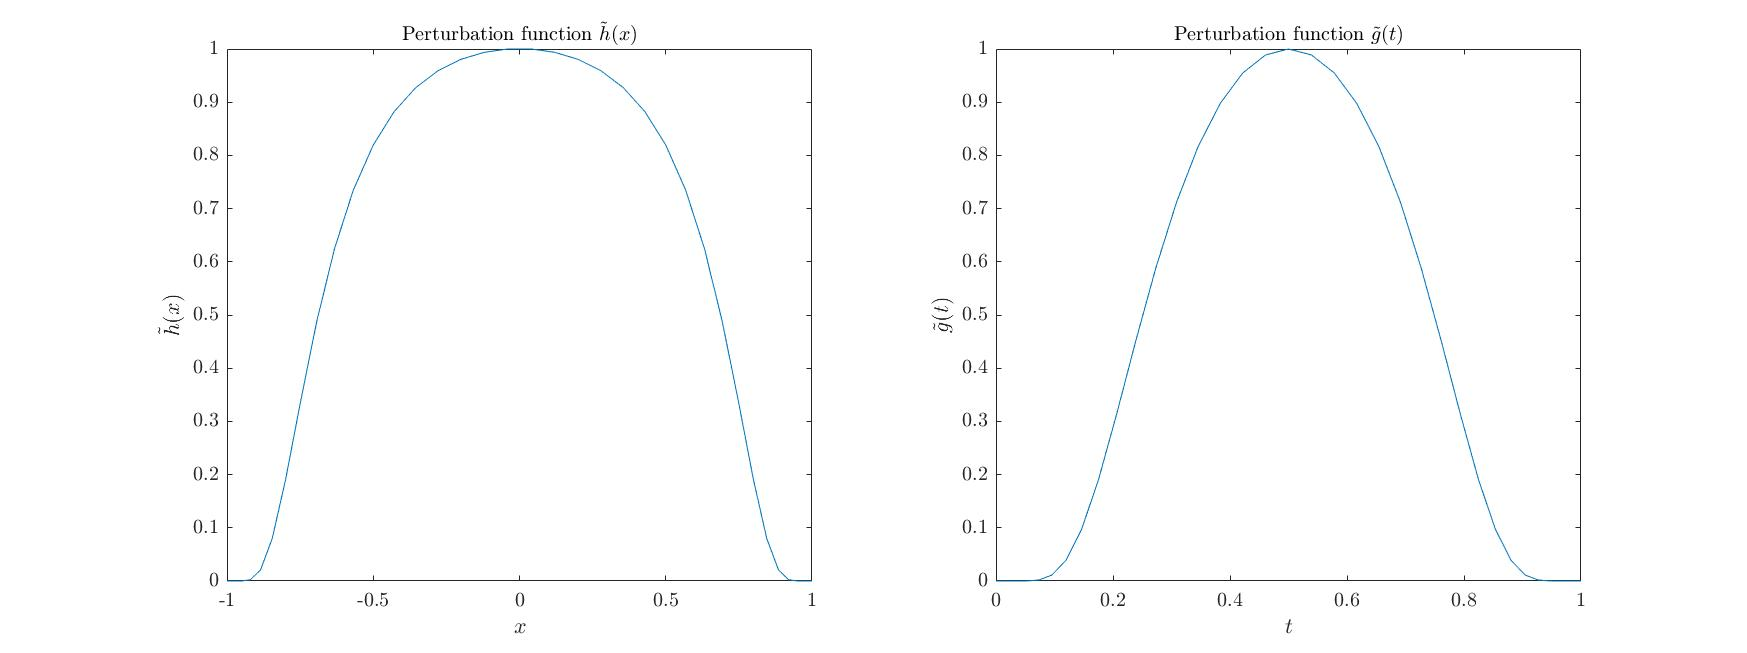
\includegraphics[scale=0.25]{PerturbationFunctions.jpg}
	\caption{Perturbation functions $\tilde h(x)$ and  $\tilde g(t)$}
	\label{Fig:PerturbationFunctions}
\end{figure} 
\begin{table}
	\begin{tabular}{ ||c |c || c || c |c | c ||}
		\hline
		                    &	& Initial Error  & Final & Error &  \\ 
		                	& $\beta$  & $\vec{w}$  & $\vec{w}$  & $\rho$ & $\adj$ \\ 
		\hline
			                & $10^{-3}$	& $0.1$  & $6.3190 \times 10^{-5}$ & $1.1648 \times 10^{-5}$ & $2.8425 \times 10^{-5}$  \\
		 $0.1\tilde g(t)$   & $10^{-1}$	& $0.1$  & $6.1449 \times 10^{-5}$ & $7.9587 \times 10^{-5}$ & $2.8405 \times 10^{-4}$ \\
		                 	& $10^{1}$	& $0.1$  & $6.1304 \times 10^{-5}$ & $7.9576 \times 10^{-5}$ & $5.8824 \times 10^{-4}$ \\
		\hline 
			                & $10^{-3}$	& $0.5$  & $2.7263 \times 10^{-4}$  & $2.9182 \times 10^{-5}$ & $3.2882 \times 10^{-5}$ \\
		$0.5 \tilde g(t)$   & $10^{-1}$	& $0.5$  & $2.7064 \times 10^{-4}$ & $2.7098 \times 10^{-4}$ &  $3.2894 \times 10^{-4}$\\
		                    & $10^{1}$	& $0.5$  & $2.7079 \times 10^{-4}$ & $2.7096 \times 10^{-4}$ & $6.8139 \times 10^{-4}$ \\
		\hline 
			                & $10^{-3}$	& $0.0855$ & $6.1809 \times 10^{-5}$ & $1.1842 \times 10^{-5}$ & $2.7355 \times 10^{-5}$ \\
		$0.1\tilde h(x)$    & $10^{-1}$	& $0.0855$ & $6.0187 \times 10^{-5}$ & $8.0212 \times 10^{-5}$ & $2.7321 \times 10^{-4}$ \\
		                    & $10^{1}$	& $0.0855$ & $6.0047 \times 10^{-5}$ & $8.0200 \times 10^{-5}$ & $5.7592 \times 10^{-4}$ \\
		\hline 
			                & $10^{-3}$	& $0.4276$  & $2.5041 \times 10^{-4}$ & $2.7429 \times 10^{-5}$ & $3.1303 \times 10^{-5}$ \\
		$0.5\tilde h(x)$    & $10^{-1}$	& $0.4276$  & $2.4833 \times 10^{-4}$ & $2.5436 \times 10^{-4}$ & $3.1332 \times 10^{-4}$ \\
	                     	& $10^{1}$	& $0.4276$  & $2.4846 \times 10^{-4}$ & $2.5435 \times 10^{-4}$ & $6.4922 \times 10^{-4}$ \\
		\hline 
    \end{tabular}
	\caption{}
\label{TabApp2}
\end{table}

\section{Comparing the fixed point algorithm with \texttt{fsolve}}
\label{app:fsolveComparison}

Example 1 in Section \ref{sec:Examples1d} is considered to compare the computational time taken of the fixed point algorithm and the inbuilt Matlab function \texttt{fsolve}. Note that the comparison is slightly impacted by the fact that convergence is measured differently in these two numerical methods. However, a general comparison can be made regarding the efficiency of the two approaches.
We choose $n=20$, $N=30$, the ODE solver tolerance is set to be $10^{-8}$, the optimality tolerance is $10^{-4}$ and $\beta = 10^{-3}$. 
As can be seen in Table \ref{TabA3:Prob1}, the running time of the fixed point algorithm is considerably faster than for \texttt{fsolve}, while the resulting values of the cost functional remain the same. This can be confirmed by comparing the number of function evaluations computed with each method, which is an important measure when dealing with large systems, such as the two-dimensional problems discussed in this paper, since each iteration is costly for large problems. The differences in $\rho$ and $\adj$ are broadly in line with the optimality tolerance set, however the control differs more because $\vec{w}$ is updated using the optimal values of $\rho$ and $\adj$. (+ Note: fsolve says: 'Equations solved, inaccuracies possible' - it never actually reached the optimality tolerance ++)

\begin{table}
\begin{tabular}{ | c | c || c | c | c ||}
\hline
\multicolumn{2}{|c||}{} & Fixed Point & \texttt{fsolve} & Difference   \\
\hline
\hline
 & $\mathcal{J}_{uc}$ & $\numprint{0.0438}$ & $\numprint{0.0438}$ &   \\
 & $\mathcal{J}_{c}$ & $\numprint{0.0011}$ & $\numprint{0.0011}$ &   \\
 & \texttt{Iter} (\texttt{funcEval}) & $\numprint{670}$ ($\numprint{670}$)  & $\numprint{38}$ ($\numprint{31959}$)  &   \\
$\kappa =-1$ & Time taken (s) & $\numprint{2.4939e+2}$ & $\numprint{9.1546e+3}$ &   \\
 & $\mathcal{E}_{\rho_{Diff}}$ & & &$\numprint{1.1348e-3}$  \\
 & $\mathcal{E}_{\adj_{Diff}}$ & & &$\numprint{7.2742e-5}$  \\
 & $\mathcal{E}_{\mathbf{w}_{Diff}}$ & & & $\numprint{7.6725e-2}$  \\
\hline
 & $\mathcal{J}_{uc}$ & $\numprint{0.0434}$ & $\numprint{0.0434}$ &   \\
 & $\mathcal{J}_{c}$ & $\numprint{0.0020}$ & $\numprint{0.0020}$ &   \\
 & \texttt{Iter} (\texttt{funcEval}) & $\numprint{654}$ ($\numprint{654}$)  & $\numprint{38}$ ($\numprint{34239}$)  &   \\
$\kappa =1$ & Time taken (s) & $\numprint{3.3794e+2}$ & $\numprint{1.0167e+4}$ &   \\
 & $\mathcal{E}_{\rho_{Diff}}$ & & &$\numprint{3.0610e-4}$  \\
 & $\mathcal{E}_{\adj_{Diff}}$ & & &$\numprint{4.8701e-5}$  \\
 & $\mathcal{E}_{\mathbf{w}_{Diff}}$ & & & $\numprint{8.9056e-3}$  \\
\hline
\end{tabular}
\caption{Comparison of the outputs of the fixed point method, with those obtained using \texttt{fsolve}.}
\label{TabA3:Prob1}
\end{table} %\label{TabA3:Prob1}
%\begin{table}[h]
%	\begin{tabular}{ ||c|| c | c | c | c |c | c | c | c ||}
%		\hline
%	        & $\gamma$ & Time taken (s) & F.Evals/Iters & $J_{FW}$ & $J_{Opt}$ & $\rho_{Diff}$ & $\adj_{Diff}$ & $\vec{w}_{Diff}$\\
%		\hline
%		Fixed Point & & $106.4930$ & $667$ & $0.0438$ & $0.0011$ & & & \\
%		\texttt{fsolve} & $-1$ & $6.3670 \times 10^4 (rerun)$ & $35384$ & $0.0438$ & $0.0011$ & & & \\
%		Difference &  &  &  &  &  & $3.3515 \times 10^{-4}$ & $1.0922\times 10^{-5}$ & $0.0076$\\
%		\hline
%		Fixed Point & & $101.4840$ & $656$ & $0.0434$ & $0.0020$ & & & \\
%		\texttt{fsolve} & $1$ & $3.3481 \times 10^4 $ & $31957$ & $0.0434$ & $0.0020$ & & & \\
%		Difference &  &  &  &  &  & $6.7721 \times 10^{-4}$ & $3.8226 \times 10^{-5}$ & $0.0204$\\
%		\hline        
%	\end{tabular}
%	\caption{Update this table eventually.}
%\label{TabApp3}
%\end{table}

\bibliographystyle{plain}
\bibliography{ParticleDynamicsPDECO}

\end{document}
